\documentclass[pdftex,10pt,b5paper,twoside]{report}
\usepackage[utf8]{inputenc}
\usepackage[acronym, toc]{glossaries}
\usepackage{biblatex}
\usepackage[colorinlistoftodos]{todonotes}
\usepackage{graphicx}
\usepackage{pgfplots}
\usepackage{fancyvrb}
\usepackage{tabularx}
\usepackage[norsk,english]{babel}
\usepackage{subfig}
\usepackage{hyperref}



\makeglossaries

\newacronym{ast}{AST}{Abstract Syntax Tree}
\newacronym{solid}{SOLID}{\textbf{S}ingle responsibility, \textbf{O}pen–closed, \textbf{L}iskov substitution, \textbf{I}nterface segregation, \textbf{D}ependency inversion}
\newacronym{dry}{DRY}{Don't Repeat Yourself}
\newacronym{srp}{SRP}{Single Responsibility Principle}
\newacronym{ocp}{OCP}{Open-Closed Principle}
\newacronym{lsp}{LSP}{Liskov Substitution Principle}
\newacronym{isp}{ISP}{Interface Segregation Principle}
\newacronym{dip}{DIP}{Dependency Inversion Principle}
\newacronym{lcom}{LCOM}{Lack of Cohesion Of Methods}
\newacronym{loc}{LOC}{Lines Of Code}
\newacronym{lloc}{LLOC}{Logical Lines Of Code}
\newacronym{mvvm}{MVVM}{Model-View-ViewModel}
\newacronym{pr}{PR}{Pull Request}
\newacronym{ntnu}{NTNU}{Norwegian University of Science and Technology}
\newacronym{mimc}{MIMC}{More Is More Complex}
\newacronym{kiss}{KISS}{Keep It Simple Stupid}
\newacronym{psi}{PSI}{Program Structure Interface}
\newacronym{dsm}{DSM}{Dependency Structure Matrix}
\newacronym{lod}{LoD}{Law of Demeter}
\newacronym{ide}{IDE}{Integrated Development Environment}
\newacronym{cli}{CLI}{Command Line Interface}
\newacronym{qa}{QA}{Quality Assurance}
\newacronym{jvm}{JVM}{Java Virtual Machine}
\newacronym{ci}{CI}{Continous Integration}
\newacronym{cc}{CC}{Cyclomatic Complexity}
\newacronym{ddpv}{DDPV}{Detection of Design Principle Violations}
\newacronym{nof}{NoF}{Number of Functions}
\newacronym{cpu}{CPU}{Central Processing Unit}
\newacronym{pm}{PM}{Project Manager}
\newacronym{api}{API}{Application Program Interface}
\newacronym{covid19}{COVID-19}{Corona Virus Disease 2019}
\newacronym{coi}{COI}{Composition over Inheritance}
\newacronym{mvp}{MVP}{Minimum Viable Product}
\newacronym{os}{OS}{Objectives of a Solution}
\newacronym{cd}{CD}{Continous Delivery}
\newacronym{os}{OS}{Objectives of a Solution}


\addbibresource{bibliography.bib}
% Development of a tool for detection of design principle violations

% Automating the code review through automatic detection of design principles 



\begin{document}



\selectlanguage{norsk}
\begin{abstract}
    Feil eller unngått bruk av designprinsipper i programvareutvikling medfører vedlikeholdsproblemer og øker utviklingskostnadene. Til nå har verktøy for utviklere i liten grad sett etter brudd på designprinsipper, og har heller ikke vært en del av arbeidsflyten til utviklere. Dette har vært grunnet vanskeligheten av å detektere brudd på designprinsipper uten å skape støy i utvikligsprosessen. Dette studiet tar en innovativ tilnærming til problemet for å se hvordan man kan lage et verktøy for deteksjon av brudd på designprinsipper som er integrert inn i arbeidsflyten til utviklere, og som ikke lider av støy. Ved å kombinere teknologi for kodeanalyse og teknologi for kvalitetssikring av kode utvikles et verktøy for deteksjon av brudd på designprinsipper med en forskningsmetode som kalles design science. Flere iterasjoner av utvikling, testing og evaluering av prototyper ble gjennomført og endte med en tidlig versjon av et \gls{mvp}. Dette produktet ble så evaluert internt og gjennom tilbakemeldinger fra open-source community. Resultatene viser at det å automatisk legge til kommentarer på \acrfull{pr} for å informere utvikleren om mulige design-problemer vil redusere innvirkningen av falske positiver, og dermed redusere støyen betraktelig sammenlignet med tidligere metoder. Dette gjør at man kan utvikle regler for deteksjon av brudd på designprinsipper med lavere krav til treffsikkerhet enn tidligere. Likevel, vanskeligheten av å detektere brudd på design-prinsipper skaper så mye falske-positiver at videre utvikling av mekanismer for å redusere støy behøves. Med videre forskning på gode heuristikker for deteksjon av brudd på designprinsipper og implementasjon av nye mekanismer for redusering av støy vil et slikt verktøy potensielt ha stor innvirkning på videre utvikling av programvare.  
    
\end{abstract}

\selectlanguage{english}
\begin{abstract}
	%Sample IMRaD abstract: 
	Absence of correctly applied design principles triggers maintainability problems in software development and increases development cost. To current date, tools for developers have to a small extent targeted design principles and have suffered from not being an integrated part of the developers workflow. The reason being the difficulties in detecting design principle violations without creating noise in the developer workflow. This study targets this problem and takes an innovative approach for investigating how one can create a tool for \gls{ddpv} that is integrated in the developer workflow without suffering from noise. By combining technologies for code analysis and \gls{qa}, a tool for \gls{ddpv} was developed using the design science methodology. Multiple iterations of development, testing and evaluation of prototypes was carried out and ended with an early version of a \acrfull{mvp}. The product was then evaluated internally and received feedback from the open-source community. The results show that using automated comments on \gls{pr} to inform the developer about possible design issues will reduce the noise from false-positives significantly. This will enable the development of rules for \gls{ddpv} with lower requirements on accuracy than what is traditionally accepted. However, the difficulty of \gls{ddpv} creates such big amount of false-positives that further development on mechanisms for reducing the noise is needed. With continued research on good heuristics for \gls{ddpv} and implementation of suggested mechanisms for reduction of noise, a tool like this this could have big implications on the maintainability of developed software. 
	
\end{abstract}
\clearpage



\tableofcontents

\cleardoublepage
\chapter{Introduction}



% https://student.unsw.edu.au/introductions - Nice resource for seeing what should be in the introdcution!

% State the general topic and give some background about its importance
Writing software that is easy to modify and extend is an important part of software engineering. Software that have these attributes (qualities) is often referred to as maintainable. Non-maintainable software is often a breeding ground for bugs, refactoring\footnote{From Wikipedia: Process of restructuring existing code without changing its external behavior \cite{refactoring}} tasks and technical debt\footnote{From Wikipedia: Concept in software development that reflects the implied cost of additional rework caused by choosing an easy (limited) solution now instead of using a better approach that would take longer \cite{technicalDebt}.}. Consequences include increased development time, inaccurate estimations causing lost deadlines and higher costs of introducing new developers to the project.

% Introduserer best practices etc. Low level code hjelp.
To help developers write code that is maintainable, well defined rules, best practices and conventions for writing code have been developed. The rules targets low-level code constructs, only covering small amounts of code. We will, refer to these as \textit{rules}.

% Introduserer høyere nivås prinsipper som angriper på et høyere nivå
Less formal design principles that targets the structure or design of code at an architectural level have also been developed. The design principles are not formal and is often open for interpretation and subject for debate. Therefore, correct appliance of the principles often requires reasoning about the business domain and predicting future changes to the code-base. 

% Introduserer hvordan verktøy kan bidra til å følge regler og prinsipper
Tools for code-analysis have been created to help developers adhere to the rules. They provide an effective way of detecting problems, and can often auto-correct or provide solutions to detected problems. The tools are ranging from separate \gls{cli}s, build plugins, native applications, online services, to \gls{ide}s and \gls{ide} plugins. Based on the use case of the tool, it is integrated into the developer workflow differently. For example directly to the developer while editing code or as automated feedback that is part of a code review.  The tools and their integration into the developer workflow have different advantages and disadvantages.

The design principles, on the other hand are mostly informal and have limited support in tools for code-analysis. According to a prestudy on the current state on tools for improvement of code quality \cite{prestudy}, the tool support for detecting violations of design principles are limited. The tools suffer from false-positives that will create an significant amount of noise during development. In addition, the existing tools are not integrated into the developer workflow, which will make the design issues appear a long time after they were introduced. Current approaches for detecting violations of design principles mostly involve manual code review, which is a time consuming and error-prone process.

% Identity the importance of the proposed research
Given the limitations in current approaches for detecting violation of design principles, more research is proposed. The importance of adhering to the design principles cannot be neglected as the architecture and design of code lay the foundation for further development. By having tools help us adhere to the design principles, we can help ensure that correct design decisions are taken and thus reduce the time required for restructuring badly designed code.  

% Present the goal and then how to reach it
The main goal of the study is to create a tool that help developers adhere to the design principles, ultimately improving the maintainability of code. By looking at existing tools, existing methods for \acrfull{ddpv}, and both advantages and disadvantages of existing developer workflows, we think it is possible to develop an effective tool for \gls{ddpv} without creating significant amounts of noise in the developer workflow.

To help with specific guidelines for development and evaluation of such a tool, the design science methodology will be followed.


The outline of the paper is as follows; Chapter \ref{background} gives some background information and an introduction to the topics maintainable code, code analysis and developer workflow. Chapter \ref{relatedwork} gives some insight in related work in the area. Chapter \ref{methodology} presents the goal of the study and the research question. Then a description of the selected research methodology and the required steps is provided. \ref{results} presents the results from developing and evaluating the prototypes. Chapter \ref{discussion} discusses the results ending with the conclusion of the study.  

\cleardoublepage
\chapter{Background}

\label{background}
To see why achieving maintainable code is important, and why a new tool for detecting design principle violations is needed, some background information is provided. We will look into what maintainable code is, how we can achieve it and how code analysis and developer workflow relates to these topics. Note that parts of sections \ref{maintainable-code} - \ref{code-analysis} is taken from the authors prestudy on the current state of tools for code analysis\cite{prestudy}, but is modified to fit the contents of this thesis.

\section{What is maintainable code?}
\label{maintainable-code}
Software maintainability is a measure of how easy it is to modify and extend existing software. It is important to notice that keeping the code maintainable is a quality that needs to be present at all stages of development, and not only in the traditional "maintenance" stage of application development.  

Software is a product that evolves over time and that continuously needs fixes, features and updates according to the customer and users needs. To make the process of developing software product cheaper we need to ensure it meets certain requirements regarding quality. It may seem counter intuitive, but high quality software is actually cheaper to produce. You can read more about this in section \ref{problem-identification-and-motiviation}. The software community is highly opinionated and software quality is measured differently based on (but not limited to) domain, programming language and business requirements. Therefore, measuring software quality and creating rules without exceptions is extremely hard. However, interestingly, the ratio of time spent reading (i.e understanding code) versus writing code is well over 10 to 1 as Robert C. Martin states in \cite{Martin:2008:CCH:1388398}. The quality of code can therefore be measured by the amount of time that is used to understand it. To reduce the amount of time spent on understanding code, we need to ensure that the written code is understandable. We need to ensure that it is easy to understand what the code does and why it does what it does. It should be easy to locate what needs to change, easy to make changes and easy to ensure that the changes does not create unwanted side effects. \hfill 
\hfill \newline

More formally, developers have defined a set of quality attributes that will help ensure that the code is of high quality. A commonly accepted collection of quality attributes include extensibility, modularity, testability, understandability, performance, reliability and security. Martin Fowler did a useful distinction using the terms \textit{internal attributes} and \textit{external attributes} \cite{internalExternal}. The distinction is whether the attribute is visible for the user or not. The internal quality attributes correspond to maintainability, that is our focus. 

Following are the definitions of the internal quality attributes with most importance in this study:
\begin{itemize}
	\item Extensibility - "Extensibility is a measure of the ability to extend a system and the level of effort required to implement the extension. Extensions can be through the addition of new functionality or through modification of existing functionality. The principle provides for enhancements without impairing existing system functions." \cite{Extensib83:online}
    	\item Modularity - "Modular programming is a software design technique that emphasizes separating the functionality of a program into independent, interchangeable modules, such that each contains everything necessary to execute only one aspect of the desired functionality." \cite{Modularp60:online}
	\item Testability - "Software testability is the degree to which a software artifact supports testing in a given test context. If the testability of the software artifact is high, then finding faults in the system (if it has any) by means of testing is easier." \cite{Software40:online}
	\item Understandability - "Understandability is defined as the attributes of software that bear on the users' (programmer) efforts for recognizing the logical concept and its applicability." \cite{Understa26:online}
\end{itemize}

In the next section we will look into methods of fulfilling these quality attributes.

\section{Achieving maintainable code}
\label{achieving-maintainable-code}
To write code that is maintainable a set of concepts, principles and conventions including; Architectural patterns, design patterns, anti-patterns, design principles, metrics and best practices is used amongst developers. Some of them are well defined, and can easily be verified through source code analysis. Others are more abstract in nature and requires reasoning from the developers and is harder to verify.

An \textit{architectural pattern} is a general, reusable solution to a commonly occurring problem in software architecture within a given context \cite{architecturalpattern}. An example is the \gls{mvvm}-pattern for mobile development \cite{mvvm}. It is a well defined pattern and correct use or misuse could be verified through testing tools like ArchUnit \cite{archunit}. 

A \textit{design pattern} is similar to an architectural pattern, but more limited in scope. An example is the Adapter pattern \cite{Adapterp54:online}. Detection of design patterns is possible through mining \cite{TEKIN2014406}. The absence of patterns is harder to detect as the absence of a design pattern is not clearly defined.

Definitions of \textit{architectural anti-patterns} and \textit{design anti-patterns} have also been made. They are the opposite of architectural-patterns and design-patterns. In other words ways one should {\em not} solve a common problem. They are commonly referred to as architecture-smells and design-smells. An example of architectural anti-pattern is the Cyclic Dependency \cite{cyclicdependency} and could be detected through dependency analysis. An example of design anti-pattern is the God-Object \cite{Godobjec14:online}, and is as stated about design patterns, not easily verifiable. However, metrics such as a high value of coupling and \gls{loc} could imply possible violations.


\textit{Design principles} are a set of guidelines that programmers should follow to avoid bad design. Because the design principles is of most importance in this study, a more in depth description is provided in section \ref{design-principles}.

\textit{Metrics} are measurements of particular characteristics of a program. They are often used as a tool for determining the code quality. Examples include cyclomatic complexity and coupling. \textit{Coupling} is the degree of interdependence between software modules \cite{coupling}. \textit{Cyclomatic complexity} is used to indicate the complexity of a program \cite{Cyclomat54:online}. They are calculated using code analysis.

\textit{Best practices} are informal rules that have been learned over time, or practice that have become part of the language ``culture''. The best practices can in some ways be equal to the design principles, but are often simpler and more limited in scope. Even if limited in scope, the range of different best practices is huge. Best practices includes but is not limited to, code patterns that are probable bugs, styling of code and readability. An example of best-practice in the Java language could be to use camel case (camelCase) \cite{camelcase} on variable-names, or to not have empty else-blocks. They are often well defined and are verified using tools for code static analysis. Tools enforcing best-practices is commonly referred to as \textit{linters}.

\section{Design principles}
\label{design-principles}
Design principles, also commonly referred to as programming principles, are a set of guidelines that programmers should follow to avoid bad design. Violation of design principles often introduces \textit{design issues}. The design issues themselves do not functionally affect the system, but will impact further development negatively. According to Robert C. Martin \cite{robertcmartinprinciples} there are three characteristics of bad design that the design principles will help reduce:

\begin{enumerate}
	\item Rigidity - It is hard to change because every change affects too many other parts of the system.
	\item Fragility - When you make a change, unexpected parts of the system break.
	\item Immobility - It is hard to reuse in another application because it cannot be disentangled from the current application.
\end{enumerate}

Having a system with any of these characteristics will drastically slow down development time, and is therefore important to fix sooner rather than later for multiple reasons. In section \ref{problem-identification-and-motiviation} we will elaborate more on this.

A common set of design principles that often is referred to is the \gls{solid} principles \cite{solid}.

\begin{itemize}
    \item \gls{srp} -- "... states that every module or class should have responsibility over a single part of the functionality provided by the software, and that responsibility should be entirely encapsulated by the class, module or function." \cite{srp}
    
    \item \gls{ocp} -- "... states "software entities (classes, modules, functions, etc.) should be open for extension, but closed for modification"; that is, such an entity can allow its behavior to be extended without modifying its source code." \cite{ocp}
    \item \gls{lsp} -- "Objects in a program should be replaceable with instances of their subtypes without altering the correctness of that program." \cite{lsp}
    \item \gls{isp} -- "... states that no client should be forced to depend on methods it does not use." \cite{isp}
    \item \gls{dip} --  "... states: \newline A. High-level modules should not depend on low-level modules. Both should depend on abstractions (e.g. interfaces). \newline
B. Abstractions should not depend on details. Details (concrete implementations) should depend on abstractions." \cite{dip}
\end{itemize}
    
As you can see, the design principles are often abstract and verification requires knowledge and reasoning about the business domain. For example, referring to the \gls{ocp}, how do you know what is going to be changed in the future, and how are you then going to design for extension? In addition, making classes closed for all modifications are not possible. And in case of the \gls{srp}, how would you determine what is a single responsibility? 

To make matters worse, the design principles may be conflicting. \gls{dip} suggests introducing abstractions to decouple software modules, while \gls{mimc} principle and \gls{kiss} principles says that introducing abstractions (e.g interfaces, abstract classes) introduces unwanted complexity. The design principles are therefore hard to verify using code analysis. The manual process of code review is therefore the main arena for detecting design issues in code.

\section{Code analysis}
\label{code-analysis}
We differentiate between two types of code analysis, dynamic code analysis and static code analysis. \textit{Dynamic code analysis} is done by analyzing programs being executed on a processor, while \textit{static code analysis} is purely based on analysis of the source code. Within static and dynamic code analysis, we could focus the analysis on either run-time properties or design time properties.

\begin{table}[h!]
\centering
\begin{tabularx}{\textwidth}{|X|X|X|}
\hline
                                & Static Analysis                                                                                        & Dynamic Analysis                                                                                       \\ \hline
Runtime properties     & \begin{tabular}[c]{@{}l@{}}- Performance \\(memory leak etc..)\\ - Correctness\\ - Security analysis\\ ...\end{tabular} & \begin{tabular}[c]{@{}l@{}}- Performance \\(memory leak etc..)\\ - Correctness\\ - Security analysis\\ ...\end{tabular} \\ \hline
Design time properties & \begin{tabular}[c]{@{}l@{}}- Design principles \\ - Style\\ - Metrics\\ ...\end{tabular}                              & - Dynamic software metrics                                                                                            \\ \hline
\end{tabularx}
\caption{A non-exhaustive table of static and dynamic analysis showing their runtime and design-time properties.}
\label{table:static-dynamic}
\end{table}

Since dynamic analysis is based on program execution it has the advantage of being able to measure the actual \gls{cpu}, memory and energy performance, and to target other dynamic aspects of programs. However, that does not mean that static code analysis is not able to target performance or dynamic aspects of source code. As seen in table \ref{table:static-dynamic} there is a great overlap between static and dynamic code-analysis. Null-pointer analysis is a form of static code-analysis that targets runtime properties of source code, without directly executing it.

As we want to improve the source code, we have chosen to focus on static code analysis with the focus on design time properties. The static analysis is done by parsing the source code, creating an \gls{ast} and then analyzing it for violations of the aforementioned principles, concepts and conventions. Some static code analysis tools also provide automatic refactoring possibilities through transformation of the \gls{ast}.


Figure \ref{fig:ast} shows a simple example \gls{ast} where a static analysis tools could detect that the expression \texttt{x == 1} always evaluates to \texttt{true} and that the variable \texttt{y} is never used. The tool could then suggest that the branching is unnecessary and that the \texttt{y} variable is removed.  

\begin{figure}[h!]
	\centering
	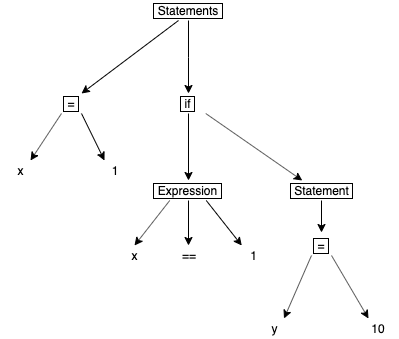
\includegraphics[width=\linewidth/2]{report/images/ast.png}
	\caption{Simple \gls{ast} of: \texttt{x=1; if (x == 1) \{y = 10;\}}}
	\label{fig:ast}
\end{figure}



\section{False-positives and false-negatives}
Because good heuristics for \gls{ddpv} is hard to define, a tool for \gls{ddpv}, would not have 100\% accuracy. The tool will therefore report violations, that in reality is not. These are false alarms and we call these \textit{false-positives}. We generally would like the rate of false-positives to be as low as possible. A \textit{false-negative} is the opposite, when actual violations goes undetected. We generally also want to keep this rate as low as possible. Together the rate of false-positives and the rate of false-negatives will determine the accuracy of detection. 

Definition of \textit{true-positives} and \textit{true-negatives} also exists. They are the counterpart of the above definitions. True-positives are the proportion of actual violations that are correctly detected. True-negatives are the proportion of actual non-violations that is not reported. In other words, that violations that does not exist is not reported. 

%It is believed that the higher the importance of the rule, the higher false-positive rate we can accept. 


\section{Code review}
\label{code-review}
Code review is a manual inspection process of looking through code. It is currently the most common way of finding design issues in code. Code review works well if done correctly, but unfortunately it is prone to human error, and doing thorough reviews are time consuming.

There are many things to consider when doing a code review. Google even maintains their own list of what to look for in a code review \cite{google-codereview}. A few bullet points is listed below.

\begin{itemize}
    \item Is the solution following the preferred coding style? Are best practices concerning design principles followed?
    
    \item Is the solution well architected? Is it following the architectural model of the application? Are all the files in the correct modules?
    
    \item Will the changes cause unexpected behavior, and break other parts of the system? 
    
    \item Is the code understandable? Does all variables, method names, classes express its intent?
    
     \item Is duplicate code introduced? Is this way of solving the problem the way we prefer it to be in this project?
\end{itemize}

When dealing with large amounts of changed code it is easy to forget some of the bullet points above. An article by Gregory Szorc\cite{gregory}, points out that "Research by Google, Microsoft and others has shown an inverse correlation with review unit size and defect rate." This means that the number of false-negatives (i.e the amount of undetected issues) usually increase as the number of changed lines in a \gls{pr} increases. Luckily, tools will be able to help us with some of the tasks regarding style and best practices. The rest have to be targeted by manual inspection of the source code. Tools should therefore help us by automating most tasks, such that the manual review is focused on finding issues that tools are not able to detect. 

By detecting issues during code review design defects will be resolved quicker because the developer can fix the issue right away. And fixing issues right away, saves a lot of time.

\section{Developer workflow}

Developers have their own workflows which they find useful, and a tool for code-analysis needs to fit the workflow to help the developer during development. There exists a number of places where a tool could be executed in the coding phases of development. Common examples include:
\begin{itemize}
    \item While coding (Tool runs continuously as the developer types)
    \item On building the application 
    \item On commit (When one bulk of changes is done)
    \item Before \gls{qa} and code review (Often in a \gls{ci} environment)
    \item Anytime the developer wants to execute the tool
\end{itemize}

Depending on the use case and the importance of the tool, the tool executes in different phases. The compiler (parser) would for example execute its code-analysis to find syntax errors on every build. Reporting issues as early as possible may generally seem like a good idea, but could distract the developer from solving the problem at hand. Especially, if the tool itself creates noise (by introducing false-positives or takes a significant amount of time to execute) reporting issues early in the development phases would annoy the developer. Simple and advanced analysis and automatic refactoring options is often included and continuously executed inside more advanced \gls{ide}'s. Examples include data-flow analysis, dead-code detection, null-pointer-analysis and automatic transformation of imperative expressions to functional expressions. These forms of analysis will often help more than annoy the developer by providing automatic fixes and giving immediate feedback. More resource heavy analysis include dynamic analysis, that searches to find performance or security issues. These kinds of tools are typically executed at a later stage, for example before a code review.

Developers also have their own preferences for workflows and when to execute and use tools. Making a tool configurable or fit in multiple execution points in the development process is therefore often appreciated.

\section{Prototyping}
Prototyping is an important activity to get feedback from users as early as possible, to better understand the problem at hand, and its requirements. Prototypes are often described using the two dimensions, horizontal and vertical. \textit{Horizontal prototypes} covers a broad view of the entire system and focuses more on user interaction with the system, rather than low level details. \textit{Vertical prototypes} on the other hand focuses on the technical challenges and a small subset of functionality of the final system. Depending on the precision, or how much it looks and works like the finished product, it is either a \textit{low fidelity} or \textit{high fidelity} prototype. 

In addition to the widely used definitions of vertical and horizontal prototypes, we would like to further describe the prototypes using the visual, interaction and content dimensions. These dimensions were introduced by Kyle Murphy in his article about describing prototypes \cite{prototype-dimensions}. The five dimensions of prototype fidelity are therefore visual, interaction, breadth, depth and content.

\begin{itemize}
    \item The \textit{visual} dimension describes how much the prototype looks like the finished product. 
    \item The \textit{interaction} dimension describes the level of interactivity the prototype has. 
    
    \item The \textit{breadth} dimension describes how much of the final products surface area that is covered. 
    
    \item The \textit{depth} dimension describes to what degree the user is constrained at a given level of breadth.
    
    \item The \textit{content} dimension describes to what degree the content (data) in the prototype represents the data that will exist in the final product.     
\end{itemize}

By creating prototypes with different focus on the dimensions, one is exploring the problem domain and will learn and understand the requirements of a solution.
\cleardoublepage
\chapter{Related work}
\label{relatedwork}

% General about tools that is related
To the best of my knowledge, a tool that directly targets the detection of violations of design principles, does not exist. There exists a lot of tools for code analysis, PMD\cite{pmd}, SonarQube\cite{sonarqube} to name two of the most used ones for the Java language. Most of them support detection of violations of style conventions, best practices and finding possible bugs. However, some tools and linters include functionality for detecting violations on a small subset of the design principles. Therefore, developers need to adopt a large suite of tools to only be able to support detection of a few design principles violations. Also, the tools are fundamentally different and have different purpose and supports integration in the development process differently. The tools are ranging from separate \gls{cli}s, native applications, online services, \gls{ide}s and \gls{ide} plugins. The purpose also varies. Some are used for project level analysis activities, for finding areas in the code-base with issues, while other tools are focused at reporting issues at the time of writing or in the \gls{qa} process. 

This thesis is mainly considering two research areas, code-analysis and code-review. First, related work on code-analysis regarding detecting design principle violations will be presented. Then other related work and tools related to code review will be presented.

PMD \cite{pmd} is one of many tools that calculates multiple metrics to indirectly support detecting design issues. Examples of metrics could be \gls{loc}, \gls{cc} and \gls{nof}. The principle of \textbf{High Cohesion - Low Coupling} is a principle that has support in multiple tools, in the form of calculating a metric, including but not limited to JArchitect \cite{jarchitect} and CodeMR \cite{codemr}. JArchitect \cite{jarchitect} also includes functionality for visualizing High Cohesion - Low Coupling using a \gls{dsm}. Another example of indirectly detecting design principle violations by using metrics is JArchitect. JArchitect uses the \gls{dsm} to find violations of \textbf{\gls{srp}} by looking at how many different types a class uses. Ndepend \cite{ndepend} calculates the \gls{lcom} value to find whether the class is cohesive or not, and therefore possibly breaking \gls{srp}. 

IntelliJ \cite{IntelliJ} and \cite{pmd} has support for detecting violations of the \textbf{\gls{lod}} principle through extensive analysis of the source code.

Detecting similar snippets of code to find violations of the \textbf{\gls{dry}} principle is targeted by many tools including, but not limited to IntelliJ\cite{IntelliJ}, PMD\cite{pmd} and Code Climate\cite{codeclimate}. However, code can violate \gls{dry} without looking similar, and tools that can detect more complicated cases have not been found.  

Other design principles like \textbf{\gls{isp}}, \textbf{\gls{ocp}} and \textbf{\gls{lsp}} are not targeted at all in tools, but several articles and forum posts on how one can spot violations have been found. The principle of Composition over inheritance is tightly related to the \gls{lsp} and \cite{composition-over-inheritance-stackoverflow} has been useful in providing automated comments. Articles about spotting violations of the \gls{ocp} and \gls{isp} principles have also been found, and has been useful for the process of implementing rules that are not targeted in the current set of tools \cite{ocp-violations} \cite{ocp2} \cite{isp-violation} \cite{ocp3}. Also, one article in the article series written by Trisha Gee on "What to look for in a code review", targeting the \gls{solid} principles have been useful \cite{whattolookforincodereview}.  

Regarding the process of code review, services like GitHub\cite{github}\footnote{From Wikipedia: "..company that provides hosting for software development version control using Git"\cite{github-wiki}} provides useful features and integration with other tools for code review. Especially a tool called Danger\cite{danger} provides the possibility of automating comments on \gls{pr}'s. It supports development of plugins to support different kinds of automation. No tools that support finding design defects have been found, but plugins that enable such development have been found. Most notable are the plugins that enables automatic commenting on pull requests based on issues found using linters. Examples include the danger-eslint-plugin\cite{danger-eslint-plugin} and the danger-detekt-plugin\cite{danger-detekt-plugin} which enables comments on \gls{pr}'s based on warnings created by eslint\cite{eslint} and Detekt\cite{detekt}, respectively. 
\cleardoublepage

\chapter{Methodology}
\label{methodology}
The selected research methodology needs to fit the goal of the study. Therefore, the goal of the study will first be presented. The selected research methodology will then be presented together with how it contributes to reaching the goal. Then, a brief description of the different steps in the research methodology is provided. 

\section{Goals of the study}

There exists a lot of theory and knowledge on how to design and build maintainable software. The knowledge is used by the developers when writing code, and some of the knowledge could be enforced by tools for code analysis. It helps developers write systems that are maintainable. However, there exists knowledge about design principles that is not used in the current set of tools for code analysis. Design principles is not targeted with the current set of tools, because it is shown hard to detect violations of design principles with high accuracy. High false-positive rates will create noise and disturb the developer.

The main goal is to create a tool that help developers adhere to the design principles, ultimately improving the maintainability of code. By looking at existing tools, existing methods for \gls{ddpv}, and both advantages and disadvantages of existing developer workflows, we think it is possible to develop an effective tool for \gls{ddpv} without creating significant amounts of noise in the developer workflow. The first sub-goal is therefore to create a set of rules for \gls{ddpv}. The rules should be as accurate as possible, but we acknowledge that there will be a certain amount of noise that will be generated. The other sub-goal is to design a solution for how and where to integrate it in the developer workflow to reduce noise generated by false-positives. The goals and the sub-goals are summarized below:

\begin{enumerate}
    \item [(\(G_1\))]  Create a tool for \gls{ddpv} to help developers write maintainable code
    \begin{enumerate}
        \item [(\(G_{1.1}\))] Create a set of rules for \gls{ddpv}
        \item [(\(G_{1.2}\))] Designing a solution for how and where to integrate it in the developer workflow to reduce noise generated by false-positives.
    \end{enumerate}
\end{enumerate}

%Avgrensning
Other quality aspects of tools such as performance and usability will not be considered important, unless it directly contributes to achieving the goals of the study. 


\section{Research methodology}
To reach the goals it will be necessary to have a practical approach where an innovative product is designed, developed and evaluated. As the goal is to help developers create more maintainable code, it is also necessary to have a user-centered approach for evaluating the product. A traditional agile user-centered design process would be a usual choice for such development. However, for this study the end product should also provide a general contribution to the research field of improving maintainability of code. The contribution should include what is learned in the process, to see if such an approach could be put more work into and possibly being a new way of helping developers create maintainable software. The Design Science research methodology fits that purpose. It is presented in (A Design Science Research Methodology for Information Systems Research) \cite{Peffers2007ADS}.

% About the chosen methodology
Design science is a research methodology that focuses on getting knowledge about a domain through development of innovative artifacts. The methodology provides specific guidelines for evaluation and iteration in research projects. The software artifact will be created through a series of iterations that include the following activities: Problem identification and motivation, definition of objectives of a solution, design and development, demonstration, evaluation and communication. Figure \ref{fig:designScience} is taken from Peffers. K \cite{Peffers2007ADS} and shows the process of the design science methodology. 

\begin{figure}[h!]
    \centering
    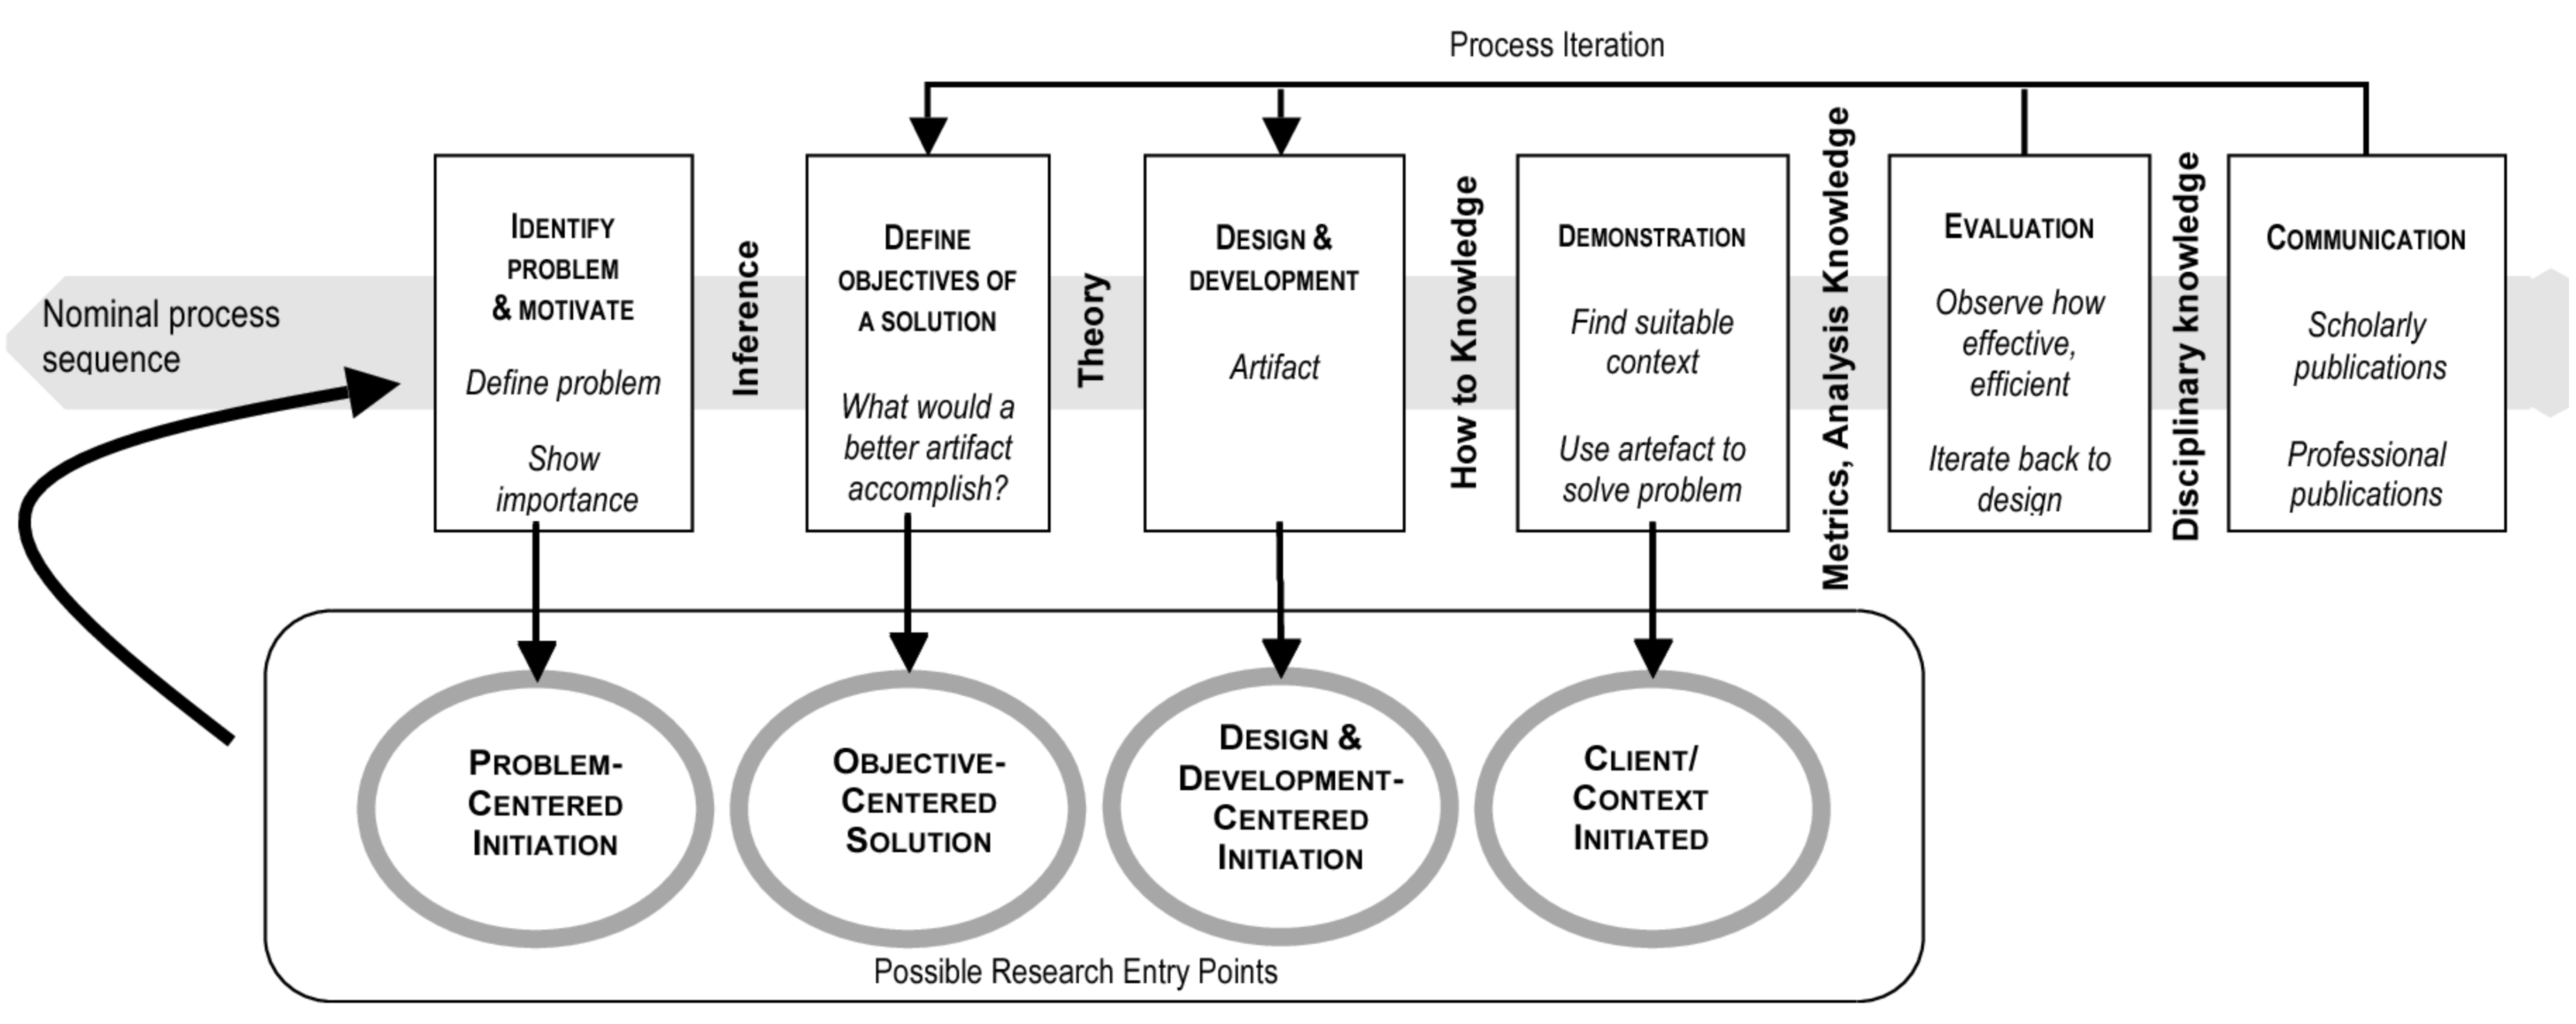
\includegraphics[width=\textwidth]{report/images/designScience.png}
    \caption{The process of the design science research methodology.}
    \label{fig:designScience}
\end{figure}

As can be seen in the figure, the activities are not required to be done in any strict order, but in the order as seen required. For example, at any point in the process, one could take a step back and redefine the objectives of a solution when new insights into the problem domain is gained. We will elaborate on how each of the different activities is applied to the study below. 

\section{Problem identification and motivation}
\label{problem-identification-and-motiviation}

% Motivation for detecting design issues is that it is cheaper to develop high quality code
As Martin Fowler explains in his article "Is High Quality Software Worth the Cost?"\cite{is-high-quality-softaware-worth-it}, the common trade-off between quality and cost does not apply to software. High quality software is actually cheaper to produce. As Martin Fowler explains in his article:

\begin{quote}
    ``Neglecting internal quality leads to rapid build up of cruft\footnote{Cruft is the difference between how the system is, and how it ideally would be.}, which slows down feature development. Even great teams produces cruft, but by keeping internal quality high, one is able to keep it under control. High internal quality keeps cruft to a minimum, allowing a team to add features with less effort, time, and cost."
\end{quote} 
It is visualized in figure \ref{fig:internal-quality-graph} which is taken from the same article. The rapid increase in cruft comes from the consequences of neglecting internal quality attributes. As discussed in section \ref{achieving-maintainable-code} an essential part of developing software with high internal quality software is to follow or adhere to the design principles. Andy Glover \& Matt Archer have written an article with 10 arguments why you should fix bugs as soon as you find them\cite{10reasons}, and the same arguments applies to design defects. Below is a short summary of the most important arguments inspired by that article:

\begin{figure}[h!]
    \centering
    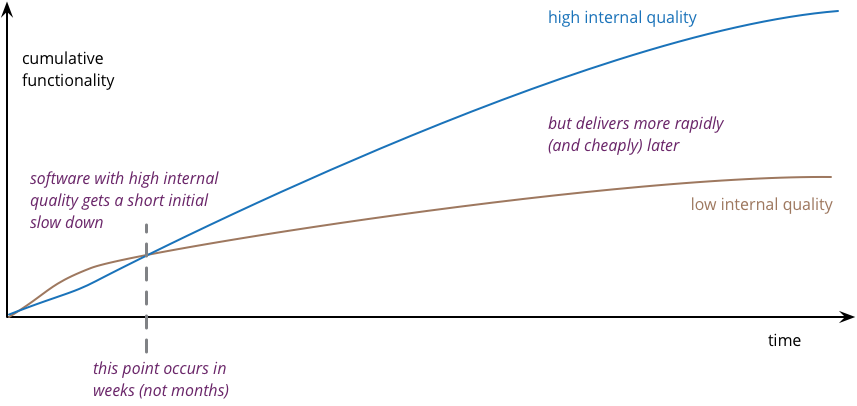
\includegraphics[width=\linewidth]{report/internal-quality-graph.png}
    \caption{Visualization of how software evolves over time, and how high/low internal quality affects development speed and cost.}
    \label{fig:internal-quality-graph}
\end{figure}

\begin{enumerate}
    \item Unfixed design defects may hide other design defects. Fixing the design defects can solve upcoming problems, that would have been harder to find at a later point.
    \item Building upon badly designed software further complicates and increases the difficulty of resolving the issues later.
  
    \item Unfixed design defects suggest internal quality is not important. If a software developer is working on poorly written software, it is likely that more code of the same style is added, continuing to degrade the system quality.
   
    \item Unfixed design defects lead to inaccurate estimates. Having design defects in code will make it hard to modify and extend the current behavior of the system. New requirements that incur changes to the code-base may break unexpected parts of the system. The estimation will then be hard to do.
   
    \item Fixing familiar code is easier than unfamiliar code. Developers need time to get familiar with code, understand what it does and why. Fixing issues while the developer is in the context of that code will save time.
\end{enumerate}

Therefore, to reduce the cruft, and thereby the cost, we should write code with high internal quality which includes adhering to design principles.

%Developers often fail to communicate the positive correlation between internal quality and development cost, which leads \gls{pm}'s to give internal quality less priority in favor of feature development.


% Motivation for helping the code review
There are mainly two techniques for detecting violations of design principles, code-analysis using tools and manual code-review. Some code-analysis tools offer design principle analysis as mentioned in section \ref{relatedwork}, but suffer from limited functionality and not being integrated into the development process. Therefore, manual code review is the main arena where most design issues are found. Finding design issues through code review is time-consuming and requires deep understanding of the problem that is being resolved. This process is prone to errors and overlooking due to human failure. Having a tool that could help this process would help to reduce the amount of design issues that will appear in production code, effectively increasing the internal quality and reducing development time and cost.

\\ The definition of the specific research problem is based on the two sub goals (\(G_{1.1}\)) and (\(G_{1.2}\)) of this study. It is as following: \textbf{How to create a tool for \gls{ddpv} that is integrated in the developer workflow without suffering from noise by false-positives?}

\section{Define the objectives of a solution}
\label{objectives-of-solution}
The objectives of a solution is initially specified based on the current knowledge about how the final product should look and be like. The objectives is then used in the evaluation of the developed prototype or artifact, and further refined based on the findings in the evaluation. This is a continuous process that will go on as long as the product is under development. The defined objectives of a solution, its specifications and refinements can be found in the results chapter.

\section{Design and development}
\label{design-development}

% Generally about design and development
The design and development phase involves the development multiple prototypes, with both high and low fidelity. To get feedback on the initial idea as quickly as possible, and then iterate and adjust the product, it is important to explore and create multiple prototypes with focus on the different dimensions. This way, the number of regressions will be reduced. Therefore, to iterate quickly, low fidelity prototypes will be created first, before gradually building more high fidelity prototypes.

The evaluation of the prototypes, why and how the different prototypes were developed is presented in the result chapter.

\section{Demonstration}

% General about demonstration. Specific demonstration details is found in results section.
The next logical step after developing a prototype is to demonstrate and test it. Depending on the prototype created, different forms of demonstration will be used. For the low fidelity prototypes, interviews and visual presentations will be used, while for the higher fidelity prototypes functional testing of the developed prototypes will be executed. 

The most important aspect of demonstrating the prototypes, is to try to create an environment that is as similar as possible to the environment that the final product will be used in. This way, the feedback will be as accurate as possible. This also involves getting users (other developers) to test the prototypes. The user group that is best suited for being informants and testers are experienced developers that have knowledge about applying and using design principles.

%Unfortunately, because a lack of resources and funding on the research project they were impossible to recruit for more in-depth evaluation. Attempts at recruiting informants for in-depth testing of the product was done by having presentations, posting on social media, creating posts in developer forums, and posting in chat groups for related tools and for work, without any luck. Additionally, the corona virus disease made physical recruitment more difficult. A conscious decision on shifting the focus to internal evaluation and feedback from open-source community was therefore seen necessary.

A description of the demonstration of each of the prototypes is found in the result chapter. 

\section{Evaluation}
% General about evaluation. Specific evaluation details is found in results section.
In the evaluation phase we will observe and evaluate how well the developed artifact solves the objectives of a solution. We will compare the artifact with the objectives of a solution, and use different techniques for evaluation based on the type of artifact and at which stage in development we are. Evaluation methods includes qualitative methods and quantitative methods. The qualitative methods include feedback gathered from having conversations with experienced developers and through presentation of prototypes. The quantitative methods include interest measurement and analysis of rule-invocations executing the final prototype on different code-bases.  

Continuous evaluation of the prototypes and the developed artifacts is important to continuously adjust the product to the users needs. After each evaluation activity, based on how the artifact compares to the objectives of a solution it is decided if another iteration is required.

The results from the evaluations is presented in the result chapter.

\section{Communication}
The last step of the design science methodology is to communicate the end result and the developed knowledge about \gls{ddpv}. The general contribution and the developed knowledge of improving the maintainability of code through \gls{ddpv} is provided through this thesis. The final artifact is available for use and further development on GitHub\cite{detekt-hint-repository}.
\cleardoublepage


\chapter{Results}
\label{results}

In this chapter we will present the results of executing multiple iterations of product development, following the design science methodology. The results of design and development are 4 different prototypes.

In section \ref{initial-os} we present the initial objectives of a solution, before giving a brief overview of the developed prototypes in section \ref{on-prototypes}. 
The prototypes are described and evaluated more in detail in sections \ref{initial-prototype}, \ref{vertical-prototype}, \ref{horizontal-prototype} and \ref{final-prototype}. The prototypes are presented and evaluated in the order the they were created. For the final prototype with the name Detekt-hint, we have dedicated a separate section (\ref{evaluation-final-prototype}) for the evaluation, which was evaluated both internally and externally using the open-source community. A description of the technical solution of the final prototype is found in section \ref{technical-solution}.

\section{Initial objectives of a solution}
\label{initial-os}
The objectives of a solution was found during multiple iterations of the design science methodology. Before each of the prototypes is presented in the next sections, we will look into the objectives of a solution that were initially specified. The initial objectives of a solution were based on the current knowledge about the domain and how the solution should be engineered to best achieve the goals. 

The first objective is that the solution should be able to detect violations of design principles using static code analysis. As discussed in the background, static code analysis is best suited for this task as we search to improve the source code itself, and not dynamic quality aspects of the code. The selection of which principles to support is based on three criteria. 

\begin{enumerate}
    \item Principles that are considered most important (i.e principles that will enable rules to detect the most major design issues) should be prioritized.
    
    \item Principles that is not targeted in existing tools should be prioritized.
    
    \item Principles that fits static code analysis should be prioritized.
\end{enumerate}

The second objective is that the solution should be designed to reduce noise from false identifications. This is based on the knowledge that current tools suffer from false-positives and that we know that the heuristics for \gls{ddpv} would not be 100\% accurate. By designing the solution to accept and reduce an amount of noise, design principles could be targeted.

The third objective is that the tool is configurable to fit team preferences at rule level. We know that developers and teams have their own preferences, and to fit different usage, the tool should be configurable. It should be possible to select which rules to enable, and to add rule-specific configuration for the different rules.

The fourth objective is that the tool should be based on an existing tool for code analysis or should be easy to integrate with existing tools. This is important for two reasons. Firstly, basing the tool on an already existing tool will drastically reduce the effort required in creating a tool for \gls{ddpv} because a framework for code analysis already will be provided. Without doing so, it would not have been feasible within the scope of this thesis. Secondly, getting users to adopt a new tool is easier if the effort required in start using the tool is low. Basing the tool on another popular tool will help getting potential users and help the ease of adoption.


The initial \gls{os} is summarized below:
\begin{itemize}
    \item [(\(OS_{1}\))] It detects violations of design principles through a set of rules using code analysis.
    \begin{itemize}
        
        \item [(\(OS_{1.1}\))] Most important design principles prioritized.
        
        \item [(\(OS_{1.2}\))] Principles that is not targeted in existing tools should be prioritized.
        
        \item [(\(OS_{1.3}\))] Design principles that fits static code analysis prioritized.
    \end{itemize}
    \item [(\(OS_{2}\))] The solution is designed to reduce eventual noise from false identifications. 
    
    \item [(\(OS_{3}\))] It is configurable. Selection of rules to enable/disable, and possibilities for configuration of individual rules.  
    
    \item [(\(OS_{4}\))] It can either be included into existing tools or is easy to integrate with existing tools.
\end{itemize}

For the individual rules there were also some specific objectives that need to be satisfied: The rules needs to be valuable, give feedback which is clear and understandable and should provide suggestions for solutions.

\section{Prototypes and development}
\label{on-prototypes}
As stated in the design and development section \ref{design-development} low-fidelity prototypes is created first, before more functional artifacts are developed. Describing the exact number of iterations and which iteration steps that were executed during development is not possible as one continuously evaluates and adjusts the product under development. However, seeing the development process in a big picture we can approximately look at 4 iterations in the design science methodology. A visualization of the general process can be seen in figure \ref{fig:workflow}.

\begin{figure}[h!]
    \centering
    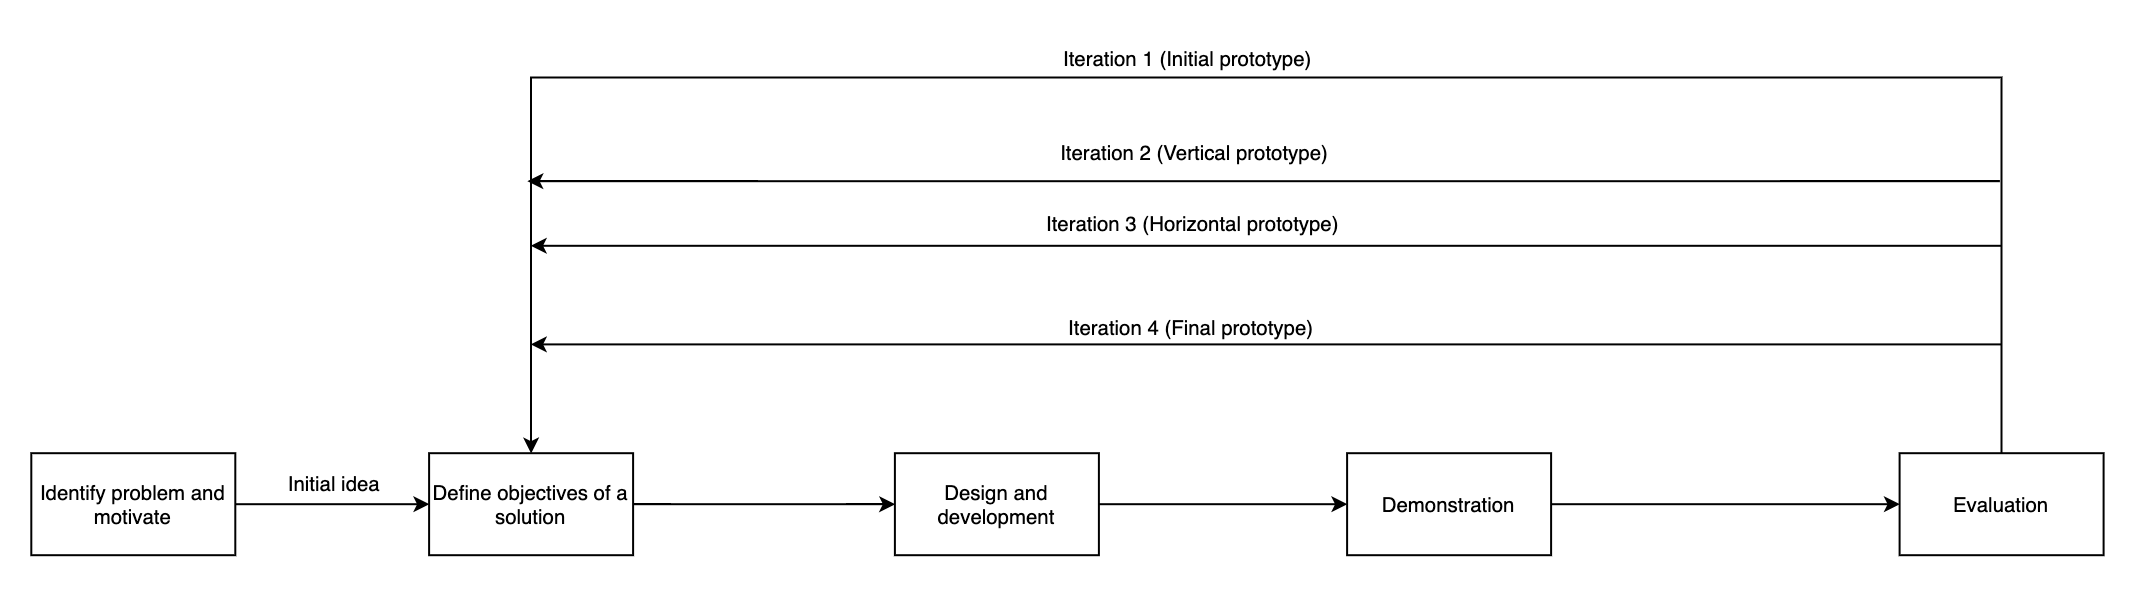
\includegraphics[width=\linewidth]{../images/workflow.png}
    \caption{The general process of development - The iterations in the design science methodology.}
    \label{fig:workflow}
\end{figure}

The 4 iterations were focused on 4 different prototypes, with both low and high fidelity, focusing on the different dimensions. An illustrative comparison of the 4 prototypes is presented in figure \ref{fig:radar-chart}. As can be seen on the figure, the development started with low fidelity prototypes, focusing on the different dimensions, and ended with the development of a high fidelity prototype. One can see that most of the dimensions were explored with high fidelity, using different prototypes. This is a positive sign, since exploration of the different dimensions is an important part of developing knowledge and understanding how the finished product should be like. 

\begin{figure}[h!]%
    \centering
    
    \subfloat[First prototype]{{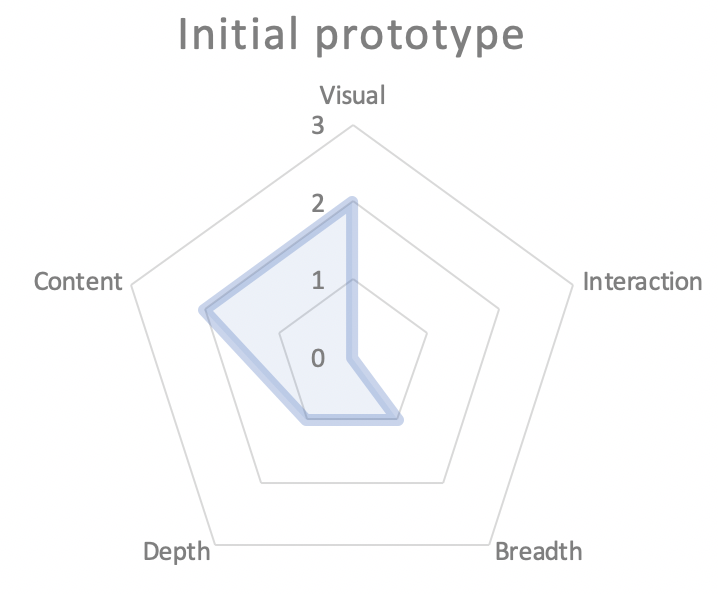
\includegraphics[width=5cm]{images/initial2.png} }}%
    \qquad
    \subfloat[Second prototype]{{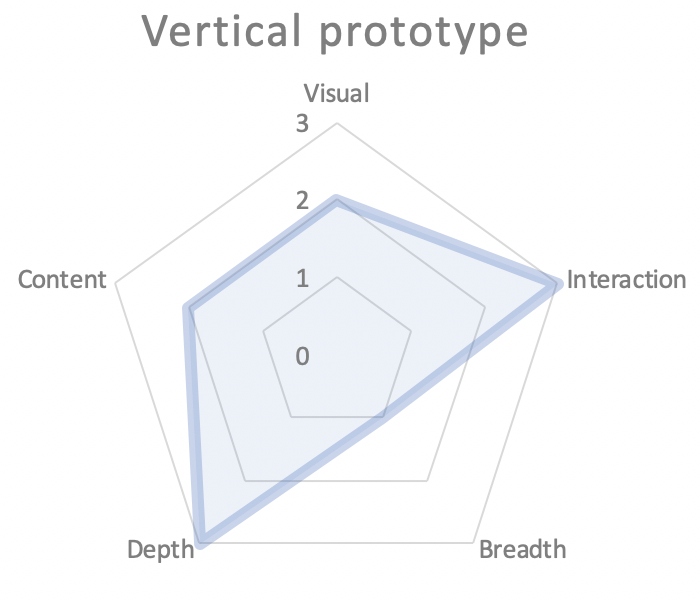
\includegraphics[width=5cm]{images/vertical2.png} }}%
    
    \subfloat[Third prototype]{{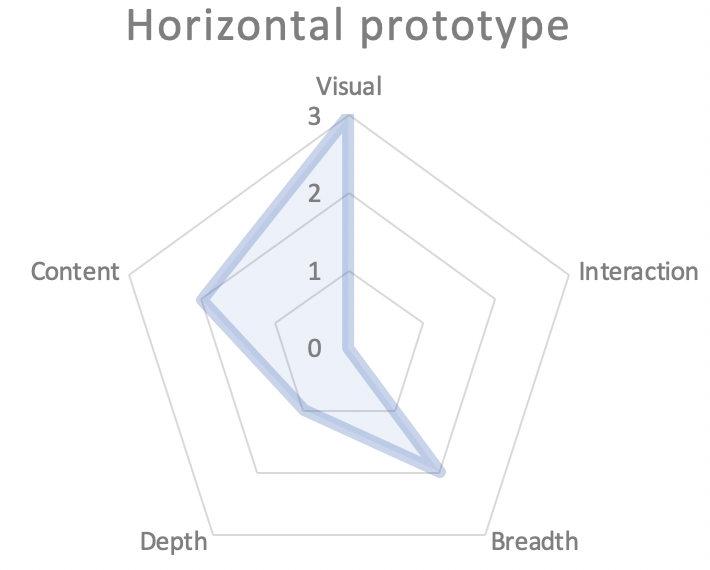
\includegraphics[width=5cm]{images/horizontal2.png} }}
    \qquad
    \subfloat[Fourth prototype]{{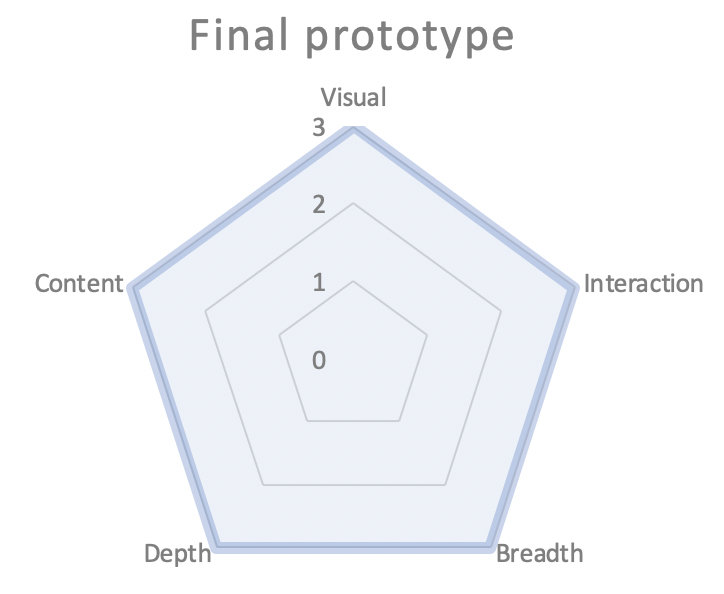
\includegraphics[width=5cm]{images/final2.png} }}
    
    
    \caption{Comparison of the 4 developed prototypes, showing the dimensions and their fidelity. The fidelity of each dimension is rated internally by the author on a scale from 0-3, where 3 is maximum of what can be expected from an early \gls{mvp}. The purpose of the comparison is solely to illustrate the different focus of each of the prototypes.}
    \label{fig:radar-chart}
\end{figure}

\section{Initial prototype}
\label{initial-prototype}
\subsection*{Why and how it was created}
An initial low resolution prototype was created first for two reasons. Firstly to see if there was any interest in a tool for \gls{ddpv}, and secondly, to start the design process of solving 
(\(OS_{2}\))\footnote{OS2: The solution is designed to reduce eventual noise from false identifications.}. The initial idea proposed a design where the tool would report design principle violations by posting comments directly in the \gls{pr}. The idea was that by having a tool that is executed just before code review, it will not cause any disturbance in early stages of development. Reporting issues in the form of comments on \gls{pr}, any false-positives would be easy to ignore and would not require any action to get rid of. This seemed like a good idea knowing that other tools for static code-analysis requires effort in suppressing false-positives, either by polluting the code-base with annotations or adding issues to a blacklist or baseline file. In addition, commenting on \gls{pr}'s will only add comments to modified/added files, which will reduce the amount of warnings that will appear.  

% Present the prototype and explain it
The prototype can be seen in figure \ref{fig:mockup}. As can be seen in figure \ref{fig:radar-chart}, the initial prototype is only an image, showing the concept. It will therefore have a low fidelity on the breadth, depth and interactivity dimensions, but has medium fidelity on the content and visual dimensions. 


\begin{figure}[h!]
    \centering
    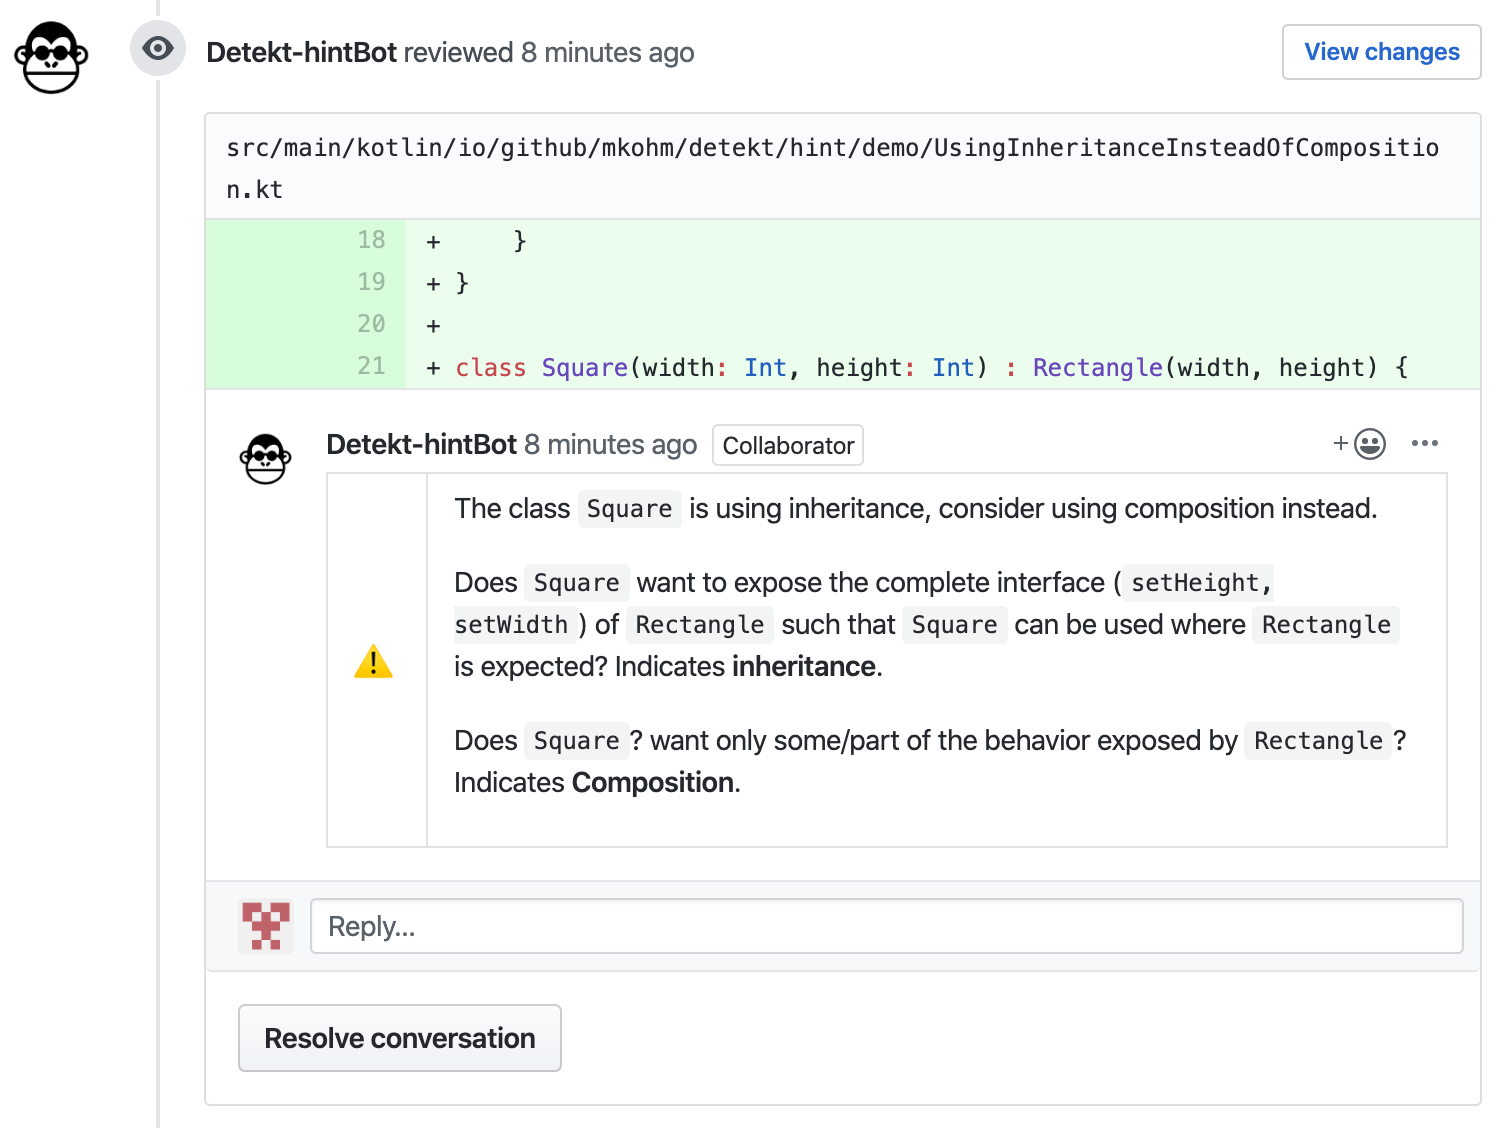
\includegraphics[width=\textwidth]{../images/demo.png}
    \caption{Initial prototype that was presented on social media and discussed with friends. The rule suggests the use of composition instead of inheritance, and helps testing if the classes adheres to the \gls{lsp}. }
    \label{fig:mockup}
\end{figure}

\subsection*{Demonstration}
The initial prototype was posted on the subreddit of Kotlin\cite{kotlin-reddit} and SoftwareArchitecture\cite{softwarearch-reddit} on Reddit. Additionally, the prototype was presented and discussed with friends. 

\subsection*{Evaluation}

The general feedback was that there was an interest in a tool like this, and that it would solve some of the issues with false-positives. It confirmed that the initial idea focused on finding a solution to (\(OS_{2}\)), should be further looked into. However, some did still point out that reducing the amount of false-positives still would be one of the most important focus points. Other suggestions for improvement included: 
\begin{itemize}
    \item Do not claim that the developer is wrong when there can be a lot of false-positives, instead present it as it \textit{might} be a violation of a design principle, and guide the developer to taking the correct decision.
    \item Identifications and even false-positives could create useful discussions within the developer team.
    \item Focus on removing the amount of false-positives as much as possible and making the product configurable to fit different needs.
  
\end{itemize}

This feedback was only based on discussions with friends and a handful of comments in the forum threads, together with a fair amount of upvotes on Reddit. In both Reddit subforums, the post received an amount of upvotes that made the post "top this week" in under 12 hours. However, the actual value of this may be limited. Read more about this in the discussion. 

For being a low resolution prototype that was created within a couple of hours, it was successful.

\section{Vertical prototype}
\label{vertical-prototype}
\subsection*{Why and how it was created}
The initial prototype proposed more work into creating a tool for detecting design principle violations, and using automated comments during code-review to reduce the amount of noise from false-positives. Normally, a horizontal prototype is built first, with the intention of getting an idea of which features that needs to be implemented and the priority of those. In this case a vertical prototype, exploring and solving the technical challenges was built first. It was built before a horizontal prototype for three reasons:

\begin{enumerate}
    \item The prioritization is somewhat known up front. Being a product focusing on detection of design principle violations, it is quite natural that the product should prioritize principles that are not covered by other tools and that the most significant principles are considered first.
    \item Too see if building a tool for \gls{ddpv} is a feasible task within the scope of a master thesis.
    \item Developers tend to be more interested in technical solutions that is working than non-interactive prototypes. Getting feedback on the following horizontal prototype would be easier if actual solutions to technical problems could be presented.
\end{enumerate}

% How the prototype was created
Before building the prototype an in depth investigation of different approaches was done. The tool would ideally support multiple languages, but to limit the scope and because of interest and knowledge about Kotlin and its ecosystem, it was selected as the language subject for analysis. Several tools and frameworks was considered to use as the fundament for a tool, including Ktlint\cite{ktlint} and Code Climate\cite{codeclimate}, but Detekt\cite{detekt} was chosen as the best platform to build on because it was made extensible, and plugins for Detekt was already existing for the automated \gls{pr} tool\cite{danger-detekt-plugin}, Danger\cite{danger}. Therefore, Detekt looked as a promising alternative for fulfillment of the objectives of a solution described in \ref{initial-os}. However, a prototype needed to be built to confirm that assumption. 

% Present and explain the prototype
Being an executable jar file, the prototype cannot be presented in this report. However, the end results of executing it looks much like the initial prototype, the only difference being that it posts comments on actual \gls{pr}'s. As can be seen in figure \ref{fig:radar-chart} the visual, breadth and content dimensions have similar fidelity as the initial prototype. Being a vertical prototype, it has higher fidelity on the depth and interaction dimensions.  

\subsection*{Demonstration}
The prototype was mainly demonstrated and continuously evaluated during development to the author. It was also partly presented to the participants at the presentation that were held for Javabin Trondheim.

\subsection*{Evaluation}
Evaluation of the vertical prototype is based on the objectives of a solution. An evaluation looking at each of the objectives is presented below.
\begin{itemize}
    \item [(\(OS_{1}\))] Using Detekt as a platform, we are able to write \gls{ddpv}-rules by analysis of the Kotlin \gls{ast} by using the Detekt rule framework and the Jetbrains \gls{psi}. Using the Detekt \gls{api} was a highly manageable task due to good documentation. However, the analysis itself using the Jetbrains \gls{psi} \gls{api} was shown to be more difficult and time consuming. Not only is it hard to create accurate heuristics for \gls{ddpv}, but it involves programming in a complex environment with a huge API with lack of documentation. In addition, creating rules for programming languages involves handling a lot of edge-cases that can take time to cover. Writing test cases for all the different scenarios ensured the proper handling of edge-cases. As development progressed the \gls{api} got more manageable and looking into other platforms or solutions for analysis were therefore not considered. However, this new knowledge about the difficulties of rule-development proposed a refinement of (\(OS_{1}\)). The adjusted objective was then as following: \\\\(\(OS_{1}\)): The tool should support a \textbf{limited} set of rules using static code analysis. \label{vertical-os1}
    
    Because of being a vertical prototype that only supported 1 rule any evaluation of the actual usefulness of the rule were not considered. This was decided to be the focus of the horizontal prototype.
    
    \item [(\(OS_{2}\))] By having a Danger integration, violations reported by the tool can be commented on pull requests, exactly as proposed in the initial prototype. The noise will therefore be significantly reduced. Code context referring to actual constructs in code can also be provided to ease the process of deciding whether an invocation is a true or false-positive. The amount and impact of false-positives can then be held to a minimum. This design will facilitate further development that will reduce the noise from false-positives. 
    
    \item [(\(OS_{3}\))] The Detekt framework provides configuration options for rules through the use of a configuration file. The rules can therefore be configured to fit the developer or teams best. The configuration file can contain custom configuration of individual rules, (e.g threshold values for rules, and files excluded from analysis). This facilitates fine grained tuning of each rule.  \label{vertical-os3}
    
    \item [(\(OS_{4}\))] The tool is easy to use with Detekt, as the developed rules for \gls{ddpv} is a Detekt rule set. However, to use the rule-set with Danger to support comments on \gls{pr}, an integration that requires a lot of additional setup and configuration is needed. This is not an optimal solution, and approaches looking to improve this should be considered. 
    
    On the plus side, all the tools and plugins that are used are open-source, making it possible for everyone to adopt the tool. \label{vertical-os4}

\end{itemize}

As a plus, even not being an objective of a solution, Detekt provides possibility for configuration to fit mainly two developer workflows. It can either be executed directly whenever the developer wants to using the \gls{cli} or Gradle task, or it can be executed before code-review using the Danger integration.

In general, it was a successful prototype that solves many of the objectives of a solution. It was a proof of concept and laid the foundations to further development. The main takeaways from evaluating the prototype was as following:
\begin{itemize}
    \item Detekt is a good platform for building such a tool and enables fulfillment of most objectives for a solution.
    \item Running the tool on own and others code is a good way of finding possible bugs and false-positives.
    \item Further development should focus on a small set of the most important rules, because they can take a long time to implement. And further evaluations of the tool need to address the usefulness of the developed rules.
\end{itemize}

\section{Horizontal prototype}
\label{horizontal-prototype}

\subsection*{Why and how it was created}
The vertical prototype showed that a limited number of rules have to be supported. That raised the question of which rules to implement and how they should support the developer in taking correct design decisions. The horizontal prototype tried to answer this question. By looking through a lot of principles, we tried to determine which rules that would be useful, and based on the feedback from the initial prototype, we wrote the comments in a way that were providing guidance instead of claiming changes because of violations. Since the \gls{solid} principles is considered by many to be the most important set of design principles, and not targeted with other tools, the focus was put on those. We also wanted to test out if a visual representation of violations of design principles is preferred or significantly better than a textual representation. Figure \ref{fig:lcom-image} shows this visual representation. The process ended by creating the horizontal prototype that included the rules that had the most value. 

The horizontal prototype was built by creating sample \gls{pr}'s in a sample repository on GitHub, and then commenting on the \gls{pr}'s with a bot user. Example images from the prototype is presented in figure \ref{fig:horizontal-prototype} and figure \ref{fig:lcom-image}. The rest of the prototype can be seen in appendix \ref{horizontal-prototype-images}. Compared to the other prototypes in figure \ref{fig:radar-chart}, this prototype is having a focus on the visuals, content and breadth dimension, while having a low depth and is non-interactive.

\subsection*{Demonstration}
Initially, to get structured feedback on the prototype, it was planned to present the prototype to a group of people using a semi structured interview. To get informants to the semi-structured interview, a presentation for approximately 20 participants at Javabin\footnote{A user group for persons interested in software development on the Java and \gls{jvm} platform, and related technologies.} Trondheim was held. Search for informants also included asking companies with Kotlin developers, including Bekk and Netlight, but with limited success. 6 participants signed up for joining the semi-structured interview, but we were only able to get in touch with 2 of them to actually join the semi structured interview. The interview followed the semi-structured interview schema that can be found in the appendix \ref{semi-structured-interview-schema}.

Due to the outbreak of \gls{covid19}, physical meetings could not be arranged, and further complicated the issue of contacting and speaking with other developers directly. We were then forced to find other ways of reaching out to people to gather feedback. The prototype were shown in multiple slack channels for work, the official Kotlin channel and various other channels.

\begin{figure}[h!]
    \centering
    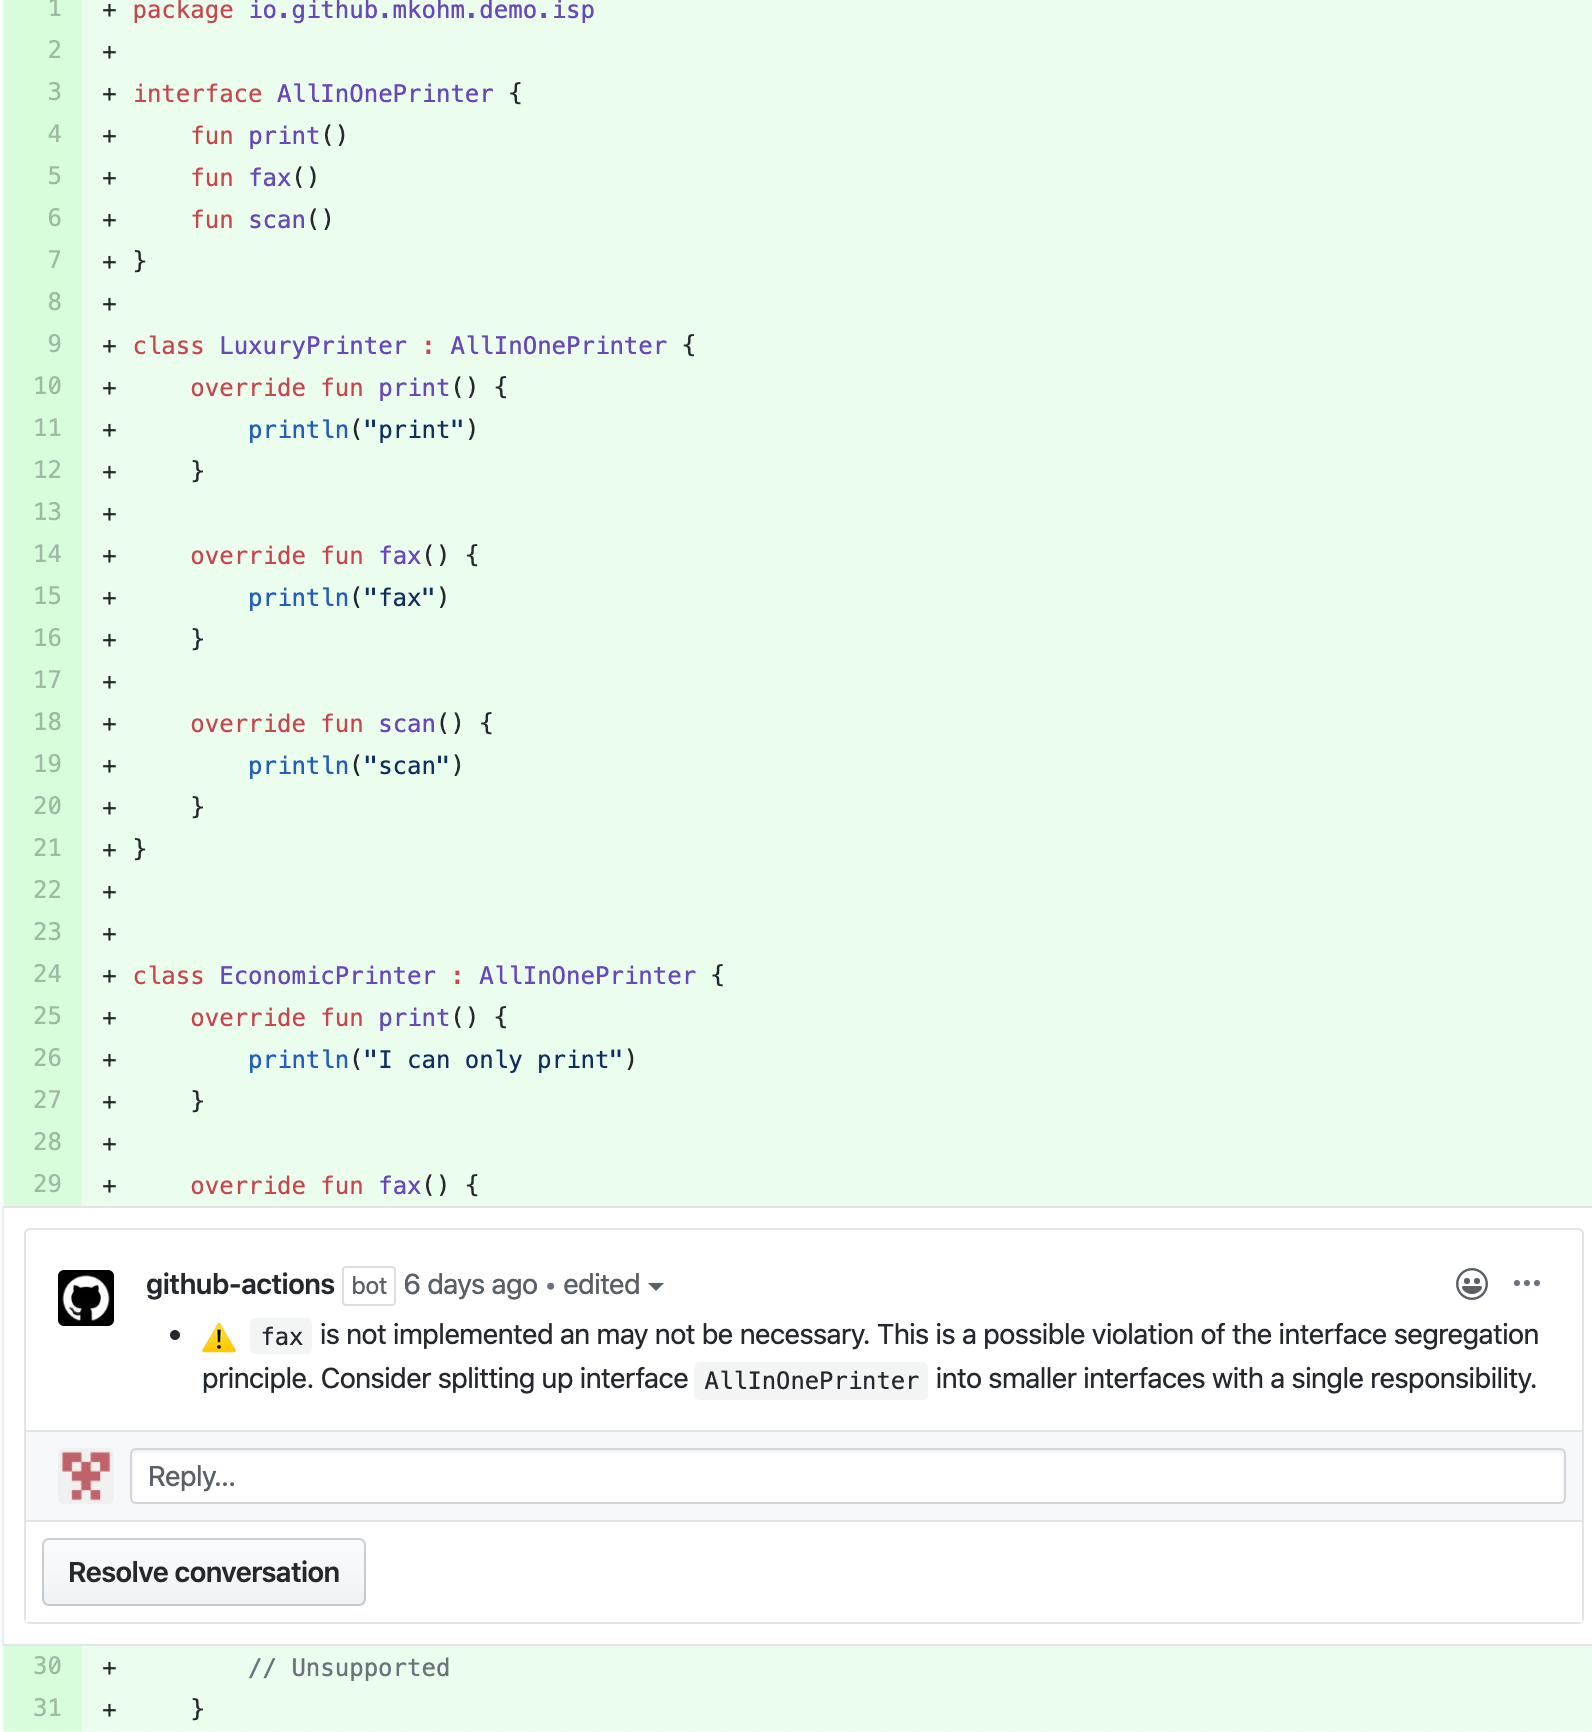
\includegraphics[width=\textwidth]{images/final_isp.png}
    \caption{Screenshot of horizontal prototype - Showing the \gls{isp} rule that has detected an empty method, which is a sign of violating the \gls{isp}.}
    \label{fig:horizontal-prototype}
\end{figure}

\begin{figure}
    \centering
    \includegraphics[width=\linewidth]{images/comment_lackOfCohesion.png}
    \caption{Screenshot of the horizontal prototype showing the \gls{lcom} rule, with a visual representation of the lack of cohesion. The figure shows which fields that are referenced from each of the methods in the class. In this case all the methods of the class references their own separate field. This indicates that each of the methods and corresponding fields have separate responsibilities within the class. This would therefore be an indication of violating the \gls{srp}.}
    \label{fig:lcom-image}
\end{figure}


\subsection*{Evaluation}

The horizontal prototype searched to answer the rule-specific objectives of a solution: If the rules would be useful, and if the comments are clear and understandable, and if they provide good suggestions for solutions to detected design issues. 

In the semi structured interview, each rule were presented and discussed. In summary the evaluation of each of the rules was:
\begin{itemize}
    \item \gls{coi} - Useful rule, but may be impacted by too many false-positives and false-negatives. Should possibly contain configuration options to exclude certain classes from analysis.
\item \gls{ocp} - Could be useful, but should further specify whether it is explicit type checking or enum switching which has triggered the invocation in the comment. 
\item \gls{isp} - Could be a useful rule, but should possibly handle Kotlin "TODO'S" specially, or would else cause some false-positives.
\item \gls{lcom} - Possibly useful. It was found out that visual representation of violations was showing useful, especially when including refactoring hints or suggestion for solutions. However, an approach generating images with refactoring hints would have much higher implementation costs than providing the same information using a textual representation. It should therefore not have first priority. More rules should be prioritized instead.
\end{itemize}

As general feedback, the rules were understandable and provided clear suggestions for solutions. However, it was suggested that reported violations should include even more context of the code (referring to actual constructs in the code) to ease the process of deciding if a detection is a true- or false-positive or to suggest fixes to the detected design issues. This resulted in a refinement of (\(OS_{2}\)). \\\\(\(OS_{2}\)) The solution is designed to reduce eventual noise from false identifications. In addition, the comments should include code context to ease the process of deciding if it is a true- or false-positive, or for suggesting fixes to design issues. \\

There was also a concern related to too few rules implemented, and that the tool would give limited value because of too few true-positives reported. Participants also mentioned that using comments in the \gls{pr} makes it easy to ignore eventual false-positives. 1 participant were more concerned about false-positives than the other.

Feedback on the prototype received through other channels than the semi-structured interview included much of the same as for the initial prototype. People like the project, and are generally positive. However, few suggestions for improvements of the developed rules or other design principles to support was received. Other features not directly related to design principles were proposed, and is written about in section \ref{futurework}.

The schema used for the semi-structured interview, the participants feedback and images of the prototype can be found in the appendix (\ref{horizontal-prototype-images}, \ref{semi-structured-interview-schema}, \ref{horizontal-prototype-interview-results}).

\section{Final prototype}
\label{final-prototype}

\subsection*{Why and how it was created}
The final prototype is a continuation of the work done on the vertical prototype, supplemented with the findings from the initial and horizontal prototype. One can consider this an early \gls{mvp}. A more technical description of the final prototype and the implemented rules is found in section \ref{technical-solution}. It can be beneficial to read that section first to get a better understanding of the developed solution.

Because the earlier prototypes gave limited amounts of feedback on the actual value of a tool for \gls{ddpv}, it was decided that the next step was to develop a functional prototype that would detect actual design issues in code, and present the findings using comments on \gls{pr}. Considering (\(OS_{1}\)) and (\(OS_{2}\)) the most important for answering the research question, the focus was put on those. Firstly, the prototype targeted OS1, by creating a set of rules for \gls{ddpv}, using the feedback from earlier prototypes. Secondly, the prototype targeted (\(OS_{2}\)), by continuing the work on designing the solution to reduce the noise from false-identifications. However, due to the outbreak of \gls{covid19}, to facilitate evaluation from the open-source community, a focus on (\(OS_{4}\)), creating a solution for easy integration into open-source projects needed to be prioritized. This unfortunately resulted in less focus on (\(OS_{1}\)) and (\(OS_{2}\)), due to unexpected integration problems, further explained in the next section. Therefore, having limited development time, not all of the received feedback received in earlier prototypes could be addressed in the final prototype. 

The final prototype consists of the same rules as the horizontal prototype, \gls{coi}, \gls{isp}, \gls{lcom} and \gls{ocp}. Images of the final prototype can be found in \ref{final-artifact}.

\subsection*{Demonstration}

Through a workshop, where participants analyze their own Kotlin code the final prototype was supposed to be evaluated. However, a new approach for evaluating the prototype had to be considered due to \gls{covid19} limiting the possibilities of meeting with other people. It was decided to focus on two types of evaluation. Evaluations based on feedback from the open-source community, and from internal analysis and testing. The evaluation from the open-source community is based on feedback gathered after having implemented the final prototype as part of the build pipeline in multiple open-source repositories on GitHub. It was created \gls{pr}'s and opened issues in multiple repositories including, Detekt\cite{detekt}, leakcanary\cite{leakcanary}, javalin\cite{javalin}, tachiyomi\cite{tachiyomi} and Tusky\cite{tusky}. It was merged for testing and used in the Javalin and Detekt repository. Unfortunately, after merging a limitation with the GitHub action API appeared. Detekt-hint did not receive write access to pull-requests to the destination repository when the build pipeline is running on the forked repository. Unfortunately, pull requests from forks is the 'de facto' way of collaborating on open-source projects on GitHub. This leaved the Detekt-hint integration almost unusable with no alternative solutions possible within the scope of this thesis. Possible solutions is presented in section \ref{possible-solutions}. Despite this limitation, it was merged for testing in the Detekt repository. The limitation made the tool only usable by members of the Detekt repository, and not contributors working on their separate forks. Using comments on \gls{pr} as a mechanism to reduce the impact of reporting false-positives could therefore only be somewhat evaluated.

The evaluation will therefore be limited to feedback from a small number of comments created on \gls{pr}'s, discussions with programmers from the open-source community and internal evaluation. The internal evaluation was based on running Detekt-hint on both known and unknown repositories measuring the amount of rule invocations and doing analysis of the actual value given by the rules. 

\section{Evaluation of the final prototype}
\label{evaluation-final-prototype}
The evaluation is divided into 5 sections. The first two sections will evaluate the tool based on the source of the feedback. Section \ref{evaluation-open-source} contains the evaluation from the open-source community, while section \ref{evaluation-internal} focuses on the internal evaluation. Section \ref{evaluation-comments} will evaluate the use of comments on \gls{pr} to reduce the impact of false-positives. Section \ref{evaluation-overall} will consider all the previous evaluations and evaluate the tool as a whole. Section \ref{evaluation-os-reference} will for the sake of completeness consider each of the defined \gls{os}, and reference to the the other evaluations mentioned above. In case the \gls{os} is not evaluated thoroughly in above sections it will be evaluated there.

\subsection{External evaluation}
\label{evaluation-open-source}
The external evaluation is based on creating issues (tickets) (with requests to create an integration with Detekt-hint) or \gls{pr}'s (actual integrations of Detekt-hint) on Github. Below we will describe the feedback received in the process of discussing and integrating Detekt-hint into open-source repositories on GitHub. 

The maintainer of the Javalin repository was positive for an integration testing out the tool. It lead to the \gls{pr} containing the integration, to be merged. It was then the GitHub Token limitation was discovered, which caused the \gls{pr} to be reverted short time after. Any feedback from running the tool on the Javalin repository was therefore not received. 

Despite the limitations with the GitHub token, it was merged and used in the Detekt repository. The tool was executed on a couple of \gls{pr}'s created by the maintainer of the Detekt repository. The feedback pointed out a too high level of noise, as well as suggestions for improving the comments and new mechanisms for reducing the noise. Some functional limitations and bugs were also discovered. In general, the feedback proposed that the tool was a too early prototype for being used without further development.

Having created an issue asking to integrate Detekt-hint on the Leakcanary project, one contributor was interested in testing out the tool on a separate fork. The owner of the repository shortly after wrote that he was more conservative than most when it comes to checks, and did not accept any false-positives. The tool were therefore not considered for integration.

The maintainer of Tusky\cite{tusky} ran the tool on the code-base using the \gls{cli} and did not find the tool particularly useful, and were generally concerned that the tool would generate too much noise. Further communication with the maintainer of Tusky revealed that they currently did not have any linter set up for their build pipeline, and that a tool discovering possible bugs and crashes would be prioritized first. Later, a tool looking for design principle violations could be looked into.

The maintainer of openhab-android\cite{openhab} read through a report from Detekt-hint finding issues on their master branch. He was also of the impression that the tool was generating too many false-positives. However, he noted that reading through the report, he found some issues that should be fixed. He especially mentioned an invocation of the \gls{ocp} rule and wondered how the code should be modified to adhere to the \gls{ocp}. We then explained and came up with a solution on what changes needed to be done. Then, a third contributor to the project mentioned that our solution may solve the problem with not adhering to \gls{ocp}, but would introduce another problem - not separating the model from the presentation. Therefore, in this case one had to consider a trade-off between adhering to the \gls{ocp} or keeping the model separated from the presentation. In this case, an agreement on model and presentation separation was considered more important. One could therefore consider this \gls{ocp}-rule invocation a false-positive.  However, there were three positive outcomes of this discussion. Firstly, the false-positive spawned a new architectural design discussion, which contributed to the observation of another design issue in the system. Secondly, the discussion contributed to knowledge sharing and learning for the involved participants.
Thirdly, this discussion was useful for the continued development of Detekt-hint, since model and presentation separation was not considered a conflicting principle with the \gls{ocp}. The false-positives could therefore lead to new insights that can be utilized for developing more accurate rules. 

Generally, it seems like the tool generates too many false-positives, making most people concerned that the tool would generate too much noise. However, due to the limitations with the integration most of the received feedback was based on running the tool on the code-base using the \gls{cli}. This is not how the tool is supposed to work, and will give the impression that the tool generates more noise than it actually will for three reasons. First, using the \gls{cli} will defeat Detekt-hint's purpose since it does not make use of the GitHub integration. Secondly, running the tool directly on the code-base without spending time configuring it, may increase the rate of invocations. Thirdly, reading through a report generated by the \gls{cli}, the rules that generates most of the noise may "destroy" the impression of the tool, making the more accurate rules less significant.

More testing of actual integrations of Detekt-hint should have been done to give better insights in the value of the tool. However, the results from the evaluation of the tool using the open-source community are quite clear. More development on reducing the noise is needed, together with a focus on resolving the discovered bugs and limitations.
 
\subsection{Internal evaluation}
\label{evaluation-internal}
\subsubsection{Rule invocations}
Six popular open-source projects including three Android apps were selected to evaluate the results of running Detekt-hint on the code-base, using the \gls{cli}. The rationale for selecting Android apps were that the author have some insights in the architecture of Android systems, and therefore true design issues could easier be verified. The other three open-source projects are the projects were the Detekt-hint integration has been discussed or opened \gls{pr} to. 


Following is a description of the open-source Kotlin projects that were selected for analysis: \textbf{Detekt} is a linter which Detekt-hint is an plugin to. \textbf{Ktor} is an asynchronous web framework for Kotlin. \textbf{Tachiyomi} is an open-source manga reader for Android. \textbf{Iosched} is an Android app from google, that is supposed to show best practices in Android development. It is believed that this app is well architecturally well designed and does not contain much design issues. \textbf{Tusky} is an Android client for the microblogging server Mastodon. \textbf{Javalin} is a Java and Kotlin web framework. 



The analysis were run with all rules enabled, default configuration and with a \gls{lcom} threshold of 0.8. To be able to compare the results from analyzing repositories for violation of design principles, any effort in specific configuration of individual rules were not done. This may result with a slightly higher rate of invocations. For example Detekt will get a higher rate of invocations for the \gls{coi} because it consists of a high number of rules, that all inherits from a base \texttt{Rule} class. Configuring the rule to ignoring the \texttt{Rule} class from this rule would have lowered the amount of invocations significantly. The results from running Detekt-hint on the aforementioned repositories is presented in the chart below. It is important to notice that even the high number of invocations it will not reflect the actual number of comments that will appear on a \gls{pr}. Comments on PR will only appear on the added or modified files.


\begin{figure}[h!]
    \centering
    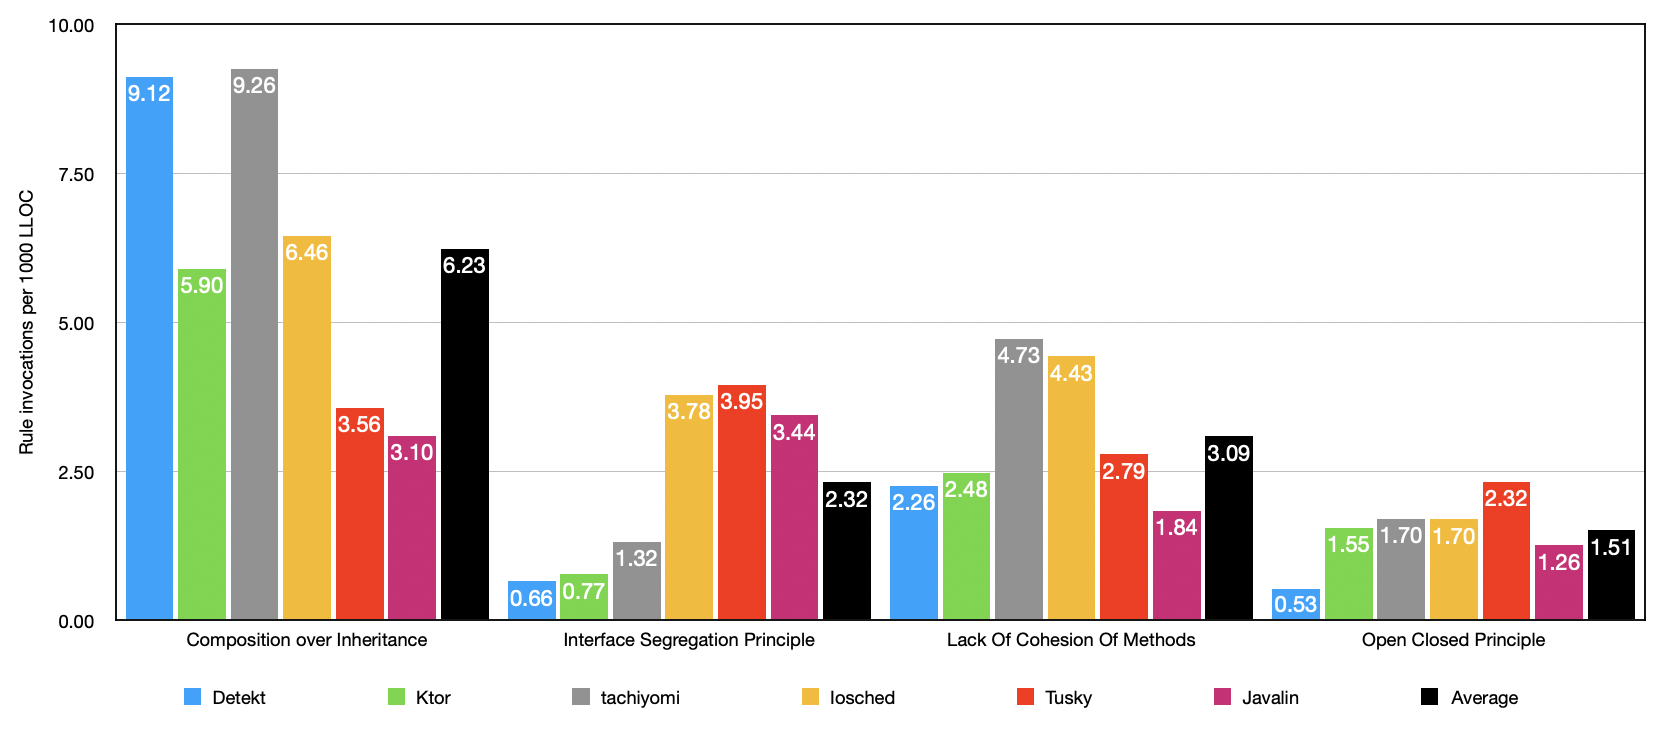
\includegraphics[width=\linewidth]{images/distribution.png}
    \caption{Number of rule invocations per 1000 \gls{lloc} for each rule, running Detekt-hint using the \gls{cli} on different repositories.}
    \label{fig:distribution}
\end{figure}


\subsubsection{Evaluation of rules}
\label{rule-evaluation}
Building on the invocations presented in the above chart, the accuracy of the tool is based on the rate of false-positives combined with the rate of false-negatives. Unfortunately, due to the nature of design principles, it is hard to know if the invocations are true or false-positives, and if there is any false-negatives without extensive knowledge about the code-base and the domain. The following evaluation of the importance and the accuracy of the rules are therefore based on simple inspections of the reported issues, without any extensive insight. The importance and accuracy of the rules is therefore rated using only three levels, low, medium and high. Note that the evaluation of the rules is based on the accuracy and importance of the rules alone, and is not considering other functional limitations that exist in the tool. Therefore, a rule itself may be considered useful, even if it is not in the current state of the tool.


\begin{itemize}

    \item \gls{coi}: Its importance is considered \textbf{high} as misusing inheritance will lead to a design with lower flexibility. The rate of false-positives is high due to reporting all occurrences of inheritance that is not from third party packages. The impact of reporting a false-positive is low due to good comments that describes the inheritance relationship and the public \gls{api} of the superclass. Together with a medium rate of false-negatives caused by not reporting issues with inheritance from third party packages, the rule has \textbf{low} accuracy. With an average rate of 6.23 invocations per 1000 \gls{lloc}, and most invocations turning out to be false-positives, the rule has room for improvement. 

    \item \gls{isp}: Its importance is considered \textbf{high} as adhering to it will help us reduce the side effects in the application and help us adhere to the \gls{srp}. The impact of reporting a false-positive is low. The rate of false-positives is low. The amount of false-negatives is high since this principle can be broken by adding new methods to interfaces, without creating empty implementations or implementations that only throws exceptions. This gives the rule a \textbf{medium} accuracy. With an average rate of 2.32 invocations per 1000 \gls{lloc}, and most invocations being true-positives, the rule is considered useful.
    
    \item \gls{ocp}: Its importance is considered \textbf{high} as it will help prevent "Shotgun surgery", altering a lot of code inside multiple classes/modules when modifying functionality. The impact of reporting a false-positive is considered low as determining whether new classes or enum entries would be introduced should be simple with some insight into the domain. The rate of false-positives is medium, and the rate of false-negatives is medium as this principle can be violated without introducing switching on enums/classes. This is giving the rule a \textbf{medium} accuracy. With an average rate of 1.51 invocations per 1000 \gls{lloc} the rule is considered useful.
    
    \item \gls{lcom}: Its importance is considered \textbf{medium}. Due to the need of finding out what is causing the cohesion to be low, the impact of reporting a false-positive is medium. Because it is controlled by the threshold value there are no false-positives and false-negatives giving the rule a \textbf{high} accuracy. However, the calculation of the \gls{lcom} value got room for improvement, due to edge cases that makes classes appear non-cohesive when they in reality are cohesive. For example it is observed that sub-classes overriding properties and methods in the parent class will get a high value of \gls{lcom} because inside the subclass, the properties are not referenced directly. With an average rate of 3.09 invocations per 1000 \gls{lloc}, the rule is considered somewhat useful, but needs further tuning and improvement on suggesting refactoring suggestions. 

\end{itemize}




\subsection{Evaluation of using comments on \gls{pr} to reduce impact of reporting false-positives}
\label{evaluation-comments}
In general, automatically adding comments to \gls{pr}'s works as a good way of exposing possible design flaws late in the development process. With informative comments that is having references to the code, possible false-positives are sorted out in a matter of seconds, and easily closed with the "resolve conversation" option. Invocation of most rules ends with informative comments, with the exception of the \gls{lcom} rule that only presents the \gls{lcom} value. However, giving a lot of context and suggestion for solutions may not always be necessary, especially after getting known with the tool. Ways of providing short succinct comments while still having the possibility of reading more about possible solutions should be looked into.

Compared to traditional linters, that would need suppression or baseline files to ignore false-positives, Detekt-hint requires no change in the source code. A false-positive requires no other further actions than pressing "resolve conversation" or simply ignoring the comment.  

Another interesting insight is that if determining whether the reported issue is a true or false-positive takes more than a few seconds it is likely that the developer did not consider the design principle during development. In that case the comment serves as a reminder and would be good for learning purposes that is constructive for further development. On the other hand, knowing that repetitive manual inspection is prone to human-failure, too many false-positives will make the developers skip the comments.

Unfortunately, the integration using comments on \gls{pr} is not problem free. Due to a limitation in Danger, the real rate of invocations per \gls{pr} is higher than what was presented in section \ref{rule-evaluation}. This is because all design issues found within a modified or added file will be added as comments to the pr, including design issues that is from lines in the analyzed file that is not present in the diff. This needs to be resolved to reduce the rate of invocations to what is presented in figure \ref{fig:distribution}.

%For illustration, a sample where detekt-hint was run on a \gls{pr} in the detekt repository showed 4 comments on a \gls{pr} with only 159 \gls{lloc} (changed minus deleted). This is similar to an invocation rate of 25, being a lot more than presented when running the cli. HHowever, these numbers are not direcly comparable due to added, modified and deleted lines of codedo not take this number for this one sample  

\subsection{Overall evaluation}
\label{evaluation-overall}

Using the numbers from the analysis of rule invocations in section \ref{evaluation-internal}, a pull request with 500 modified \gls{lloc}, having four rules enabled, with no specific configuration, will on average generate 6.6 comments on each \gls{pr}. This is not an awful lot, but considering only 4 rules, with the possibility of adding many more, it is considered too much and would lead to developers ignoring the comments. The results from the external evaluation in the open-source community confirms this. The way we see it there are mainly 4 problems with the current implementation that needs to be resolved for the tool to be useful. They are essentially refinements to (\(OS_{1}\)), (\(OS_{2}\)) and (\(OS_{3}\)). 

The first three of the problems is related to what we would like to define as "\textit{mechanisms for reducing noise}". They are mechanisms that is supporting the lack of accuracy of the developed rules.

\begin{enumerate}

    \item The final artifact should only trigger comments on changed lines of code. Currently all design issues found within a file will be added as comments to the \gls{pr}, including design issues that is from lines in the file that does not appear changed in the \gls{pr}. Only changed lines of code should get comments. Due to a limitation in Danger this was not possible to implement for this prototype.
    
    \item Detekt-hint reports the same design issues for the same files when non-functional changes are committed. For example changes related to formatting or renaming will trigger rule-invocations, while the semantics are unchanged. A mechanism that only would trigger comments on \gls{pr} if the semantics are changed would have reduced the amount of noise.
    
    \item No fine grained configuration of the rules. Currently, the configuration options for each of the rules are limited and does only include an option to exclude files from analysis. For example for the \gls{ocp} and \gls{coi} rule one could have created a configuration option to exclude a list of classes from analysis. This would however put a big strain on developers to spend a lot of time fine tuning the configuration. By introducing a way of providing configuration to the bot, the effort required for fine-tuned configuration will be much lower. The tool would then get configured over time. For example by replying to the bot or clicking pre-made reply-options this task of configuration could be semi-automated. This way we would reduce the total rate of false-positives. Analysis on the \gls{coi} rule on the Detekt repository, suggests that ignoring the superclass \texttt{Rule} (always allowing subclassing this class) one can remove 140 out of 291 invocations. For \gls{ocp} and \gls{isp} similar possibilities exist, and would further reduce the number of invocations. However, one needs to ensure that such capabilities are not misused to silence Detekt-hint, defeating the tools purpose.
    
    \item Inaccurate rules. Most rules should be improved with better heuristics for \gls{ddpv} to reduce the amount of false-invocations.
   
\end{enumerate}

All in all, even with the limitations that made integration and testing using the open-source community difficult, the final prototype was successful. It revealed many existing problems, bugs and limitations that have given insights in what needs to be resolved in future prototypes. 


\subsection{Evaluation of the objectives of a solution}
\label{evaluation-os-reference}
The final prototype being an early functional prototype, can be evaluated against all of the \gls{os} presented in section \ref{objectives-of-solution}. The evaluation of all the objectives for the final prototype is mainly covered in the above sections (\ref{evaluation-open-source}, \ref{evaluation-internal}, \ref{evaluation-comments} and \ref{evaluation-overall}). For the sake of completeness, and to make sure that each \gls{os} is evaluated, we will look at each OS, and reference to the evaluation presented above. 


%Since the final prototype is a continuation of the work done on the vertical prototype, most of the evaluation related to the technical aspects is covered in section \ref{vertical-prototype}.

\begin{itemize}
    \item [(\(OS_{1}\))] Building on the evaluation of (\(OS_{1}\)) presented in section \ref{vertical-os1}, the final prototype contains 4 rules. The \gls{solid} principles were considered the most widely known and used. Therefore, four rules adapted to support the detection of \gls{srp}, \gls{lsp}, \gls{ocp} and \gls{isp} violations were created. An evaluation of the specific rules is presented in section \ref{rule-evaluation}, and feedback on the rules from the open-source community is targeted in section \ref{evaluation-open-source}.
    
    \item [(\(OS_{2}\))] The evaluation of how good the design is for reducing the noise from false-positives is based on the mechanisms that support the rules with low accuracy. See section \ref{evaluation-comments} for evaluation of using comments on \gls{pr} to reduce noise, and section \ref{evaluation-overall} for reading about more measures that could have been taken to support the rules with low accuracy. 
    
    \item [(\(OS_{3}\))] The tool is configurable at the rule level, and can be enabled/disabled individually. There is also an option to exclude a list of files from analysis using a globing pattern. As described in \ref{rule-evaluation}, more rule-specific configuration options should be introduced to further reduce the amount of noise. In addition to being configurable at the rule level, the tool can also be executed using the \gls{cli}, making it fit other developer workflows. 
    
    \item [(\(OS_{4}\))] The final prototype can be added do any project on GitHub using GitHub Workflows, and only requires two files for being set up. This includes one configuration file for configuration of the tool, and one workflow file that will load and execute the developed GitHub Action. This is a major improvement of what was done in the vertical prototype. The tool is therefore easy to adopt, and to run as part of \gls{ci}.

\end{itemize}

\section{Technical solution}
\label{technical-solution}
To better understand the developed tool, its strength and weaknesses, implications and limitations a technical description of the tool is provided. Following is a description of the different components, ending with a description of how the different components interact to provide the ending result.

\subsection{Detekt}
Detekt is a static analysis tool for Kotlin. Detekt is comprised of a set of rules for analysis of Kotlin source code. Part of Detekt is also the Detekt-api, which gives access to a framework for creating rules, configuring rules, and for analyzing the source code. Under the hood it gives us access to IntelliJ \gls{psi} for code analysis. The PSI is built on top of the \gls{ast} provided by the Kotlin compiler, and enables modification, querying and navigation of the underlying \gls{ast}. Detekt is made extensible, and plugins (new rule-sets) can easily be added. It is easily invoked using the \gls{cli} interface.

Figure \ref{fig:psi} shows a simplified example \gls{psi} that Detekt-hint would use to find violations of \gls{isp}. The analysis would simply look in the PSI for classes that implement interfaces, and see if the overridden methods of that interface are empty or only throws exceptions. 

\begin{figure}[h!]
    \centering
    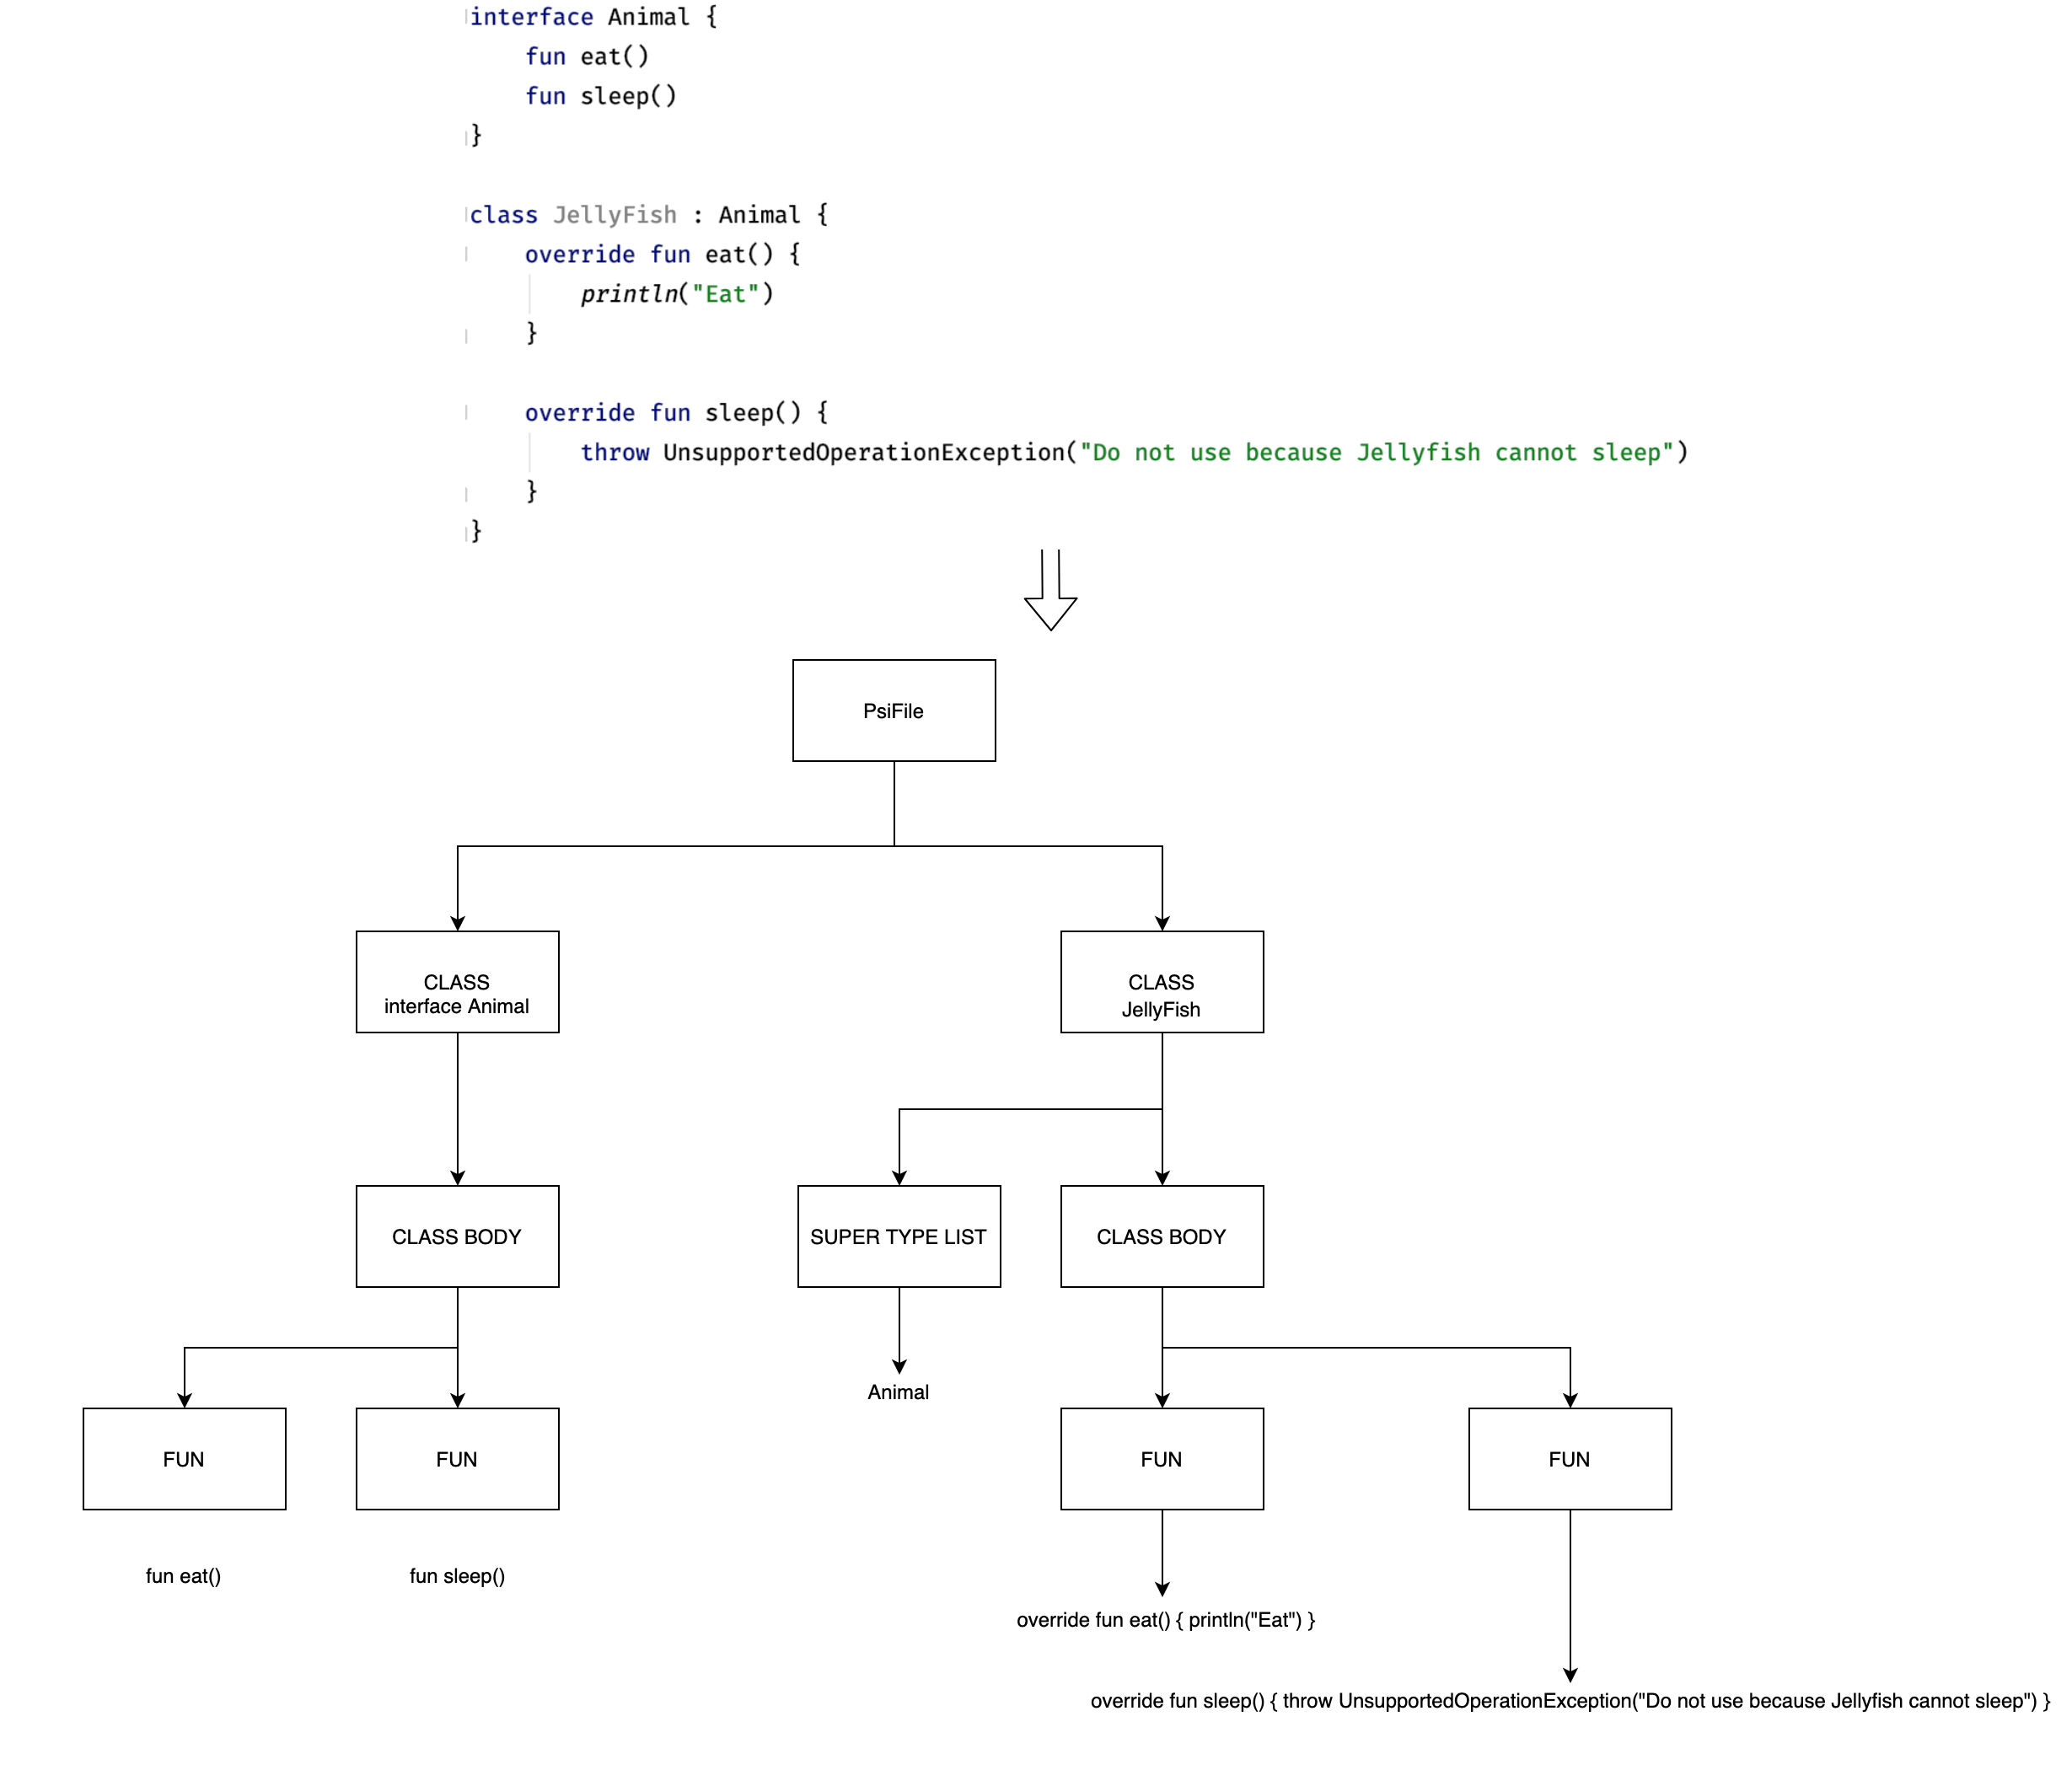
\includegraphics[width=\linewidth]{report/images/psi.png}
    \caption{Simplified version of a sample \gls{psi} showing a sign of violating the \gls{isp}.}
    \label{fig:psi}
\end{figure}

When Detekt is executed, it looks at all the rule-sets (and the configuration of them) and does analysis of the source code. When issues are found, the file and line number is noted, together with the comment to be added, and added to a report, which is the final output of the program. 

\subsection{Detekt-hint rule set}
The Detekt-hint rule set is a plugin to Detekt, and contains the implemented rules for \gls{ddpv}. The final artifact consists of four rules. The rules are described briefly below.

\begin{itemize}
    \item\gls{coi} (Liskov substitution). It promotes the use of composition instead of inheritance, since composition often allows for more flexible design \cite{composition-over-inheritance-wiki}. The rule will fire when inheritance is introduced, and help test for Liskov substitution, as presented in \cite{composition-over-inheritance-stackoverflow}. The rule will not fire if you derive from a class that exists in a third party package. This will reduce the amount of invocations significantly since some frameworks or libraries forces the use of inheritance.
    
    \item Lack of Cohesion Of Methods (LCOM). It promotes creating classes with high cohesion. The rule will detect low cohesion through a calculated metric. Low cohesion is often a sign of \gls{srp} violation, and will prevent "Shotgun surgery" \cite{lcomdescription}. \gls{lcom} for a class will range between 0 and 1, with 0 being totally cohesive and 1 being totally non-cohesive. The metric is calculated using this definition taken from \cite{lcomdescription}: "For each property in the class, you count the methods that reference it, and then you add all of those up across all properties. You then divide that by the count of methods times the count of properties, and you subtract the result from one".
    
    \item Interface Segregation Principle (\gls{isp}). It helps with reducing side-effects in the application and helps us adhere to the \gls{srp} \cite{isp-violation}. The rule looks for classes that implement methods it does not need, either by finding empty methods or methods that only throws exceptions.
    
    \item Open-Closed-Principle (\gls{ocp}). Promotes the use of abstractions to extend the functionality instead of modifying existing code to implement new behavior. This will help to reduce unwanted behavior (bugs), and prevent "Shotgun surgery" in existing code when new behavior or features are added. Violations of this principle is often spotted with long if/else chains, switching or by using abstract classes, but is checking for concrete implementations to control flow\cite{ocp3}. The rule will look for checks of concrete implementations and switching on enums inside Kotlin \texttt{when} constructs. Kotlin \texttt{when} constructs is the more powerful equivalent of Java's switch statement.
\end{itemize}

%Final source code can be found on GitHub\cite{detekt-hint-repository}. Developed as a plugin to detekt. Is built as a jar and either included in the gradle build script as a detekt plugin or run separately as a command line interface.

\subsection{Danger}
Danger is a system which is created for the purpose of automatically adding comments to \gls{pr}'s. It provides an easy to use \gls{api} for extracting the required information from Git, and provides methods for commenting on \gls{pr}'s, using a bot. It is executed in the \gls{ci} environment on every commit to \gls{pr}'s that is created. It will therefore remove the comments when the issues are resolved, to reflect the current state of the \gls{pr}. 

\subsection{GitHub Actions and the execution flow}
GitHub Actions is a tool created by GitHub for automating software workflows, including \gls{ci}/\gls{cd}. A custom GitHub Action workflow is created for Detekt-hint. When a \gls{pr} is created or updated this workflow will executes the Detekt-\gls{cli} together with the Detekt-hint rule set. This will generate the report containing all the comments to be added on the \gls{pr}. Danger is then executed and picks up the report with the comments to be added. It will then add a comment on the \gls{pr} for every comment in the file. A diagram of how everything interacts can be seen in figure \ref{fig:integration}. 


\begin{figure}
    \centering
    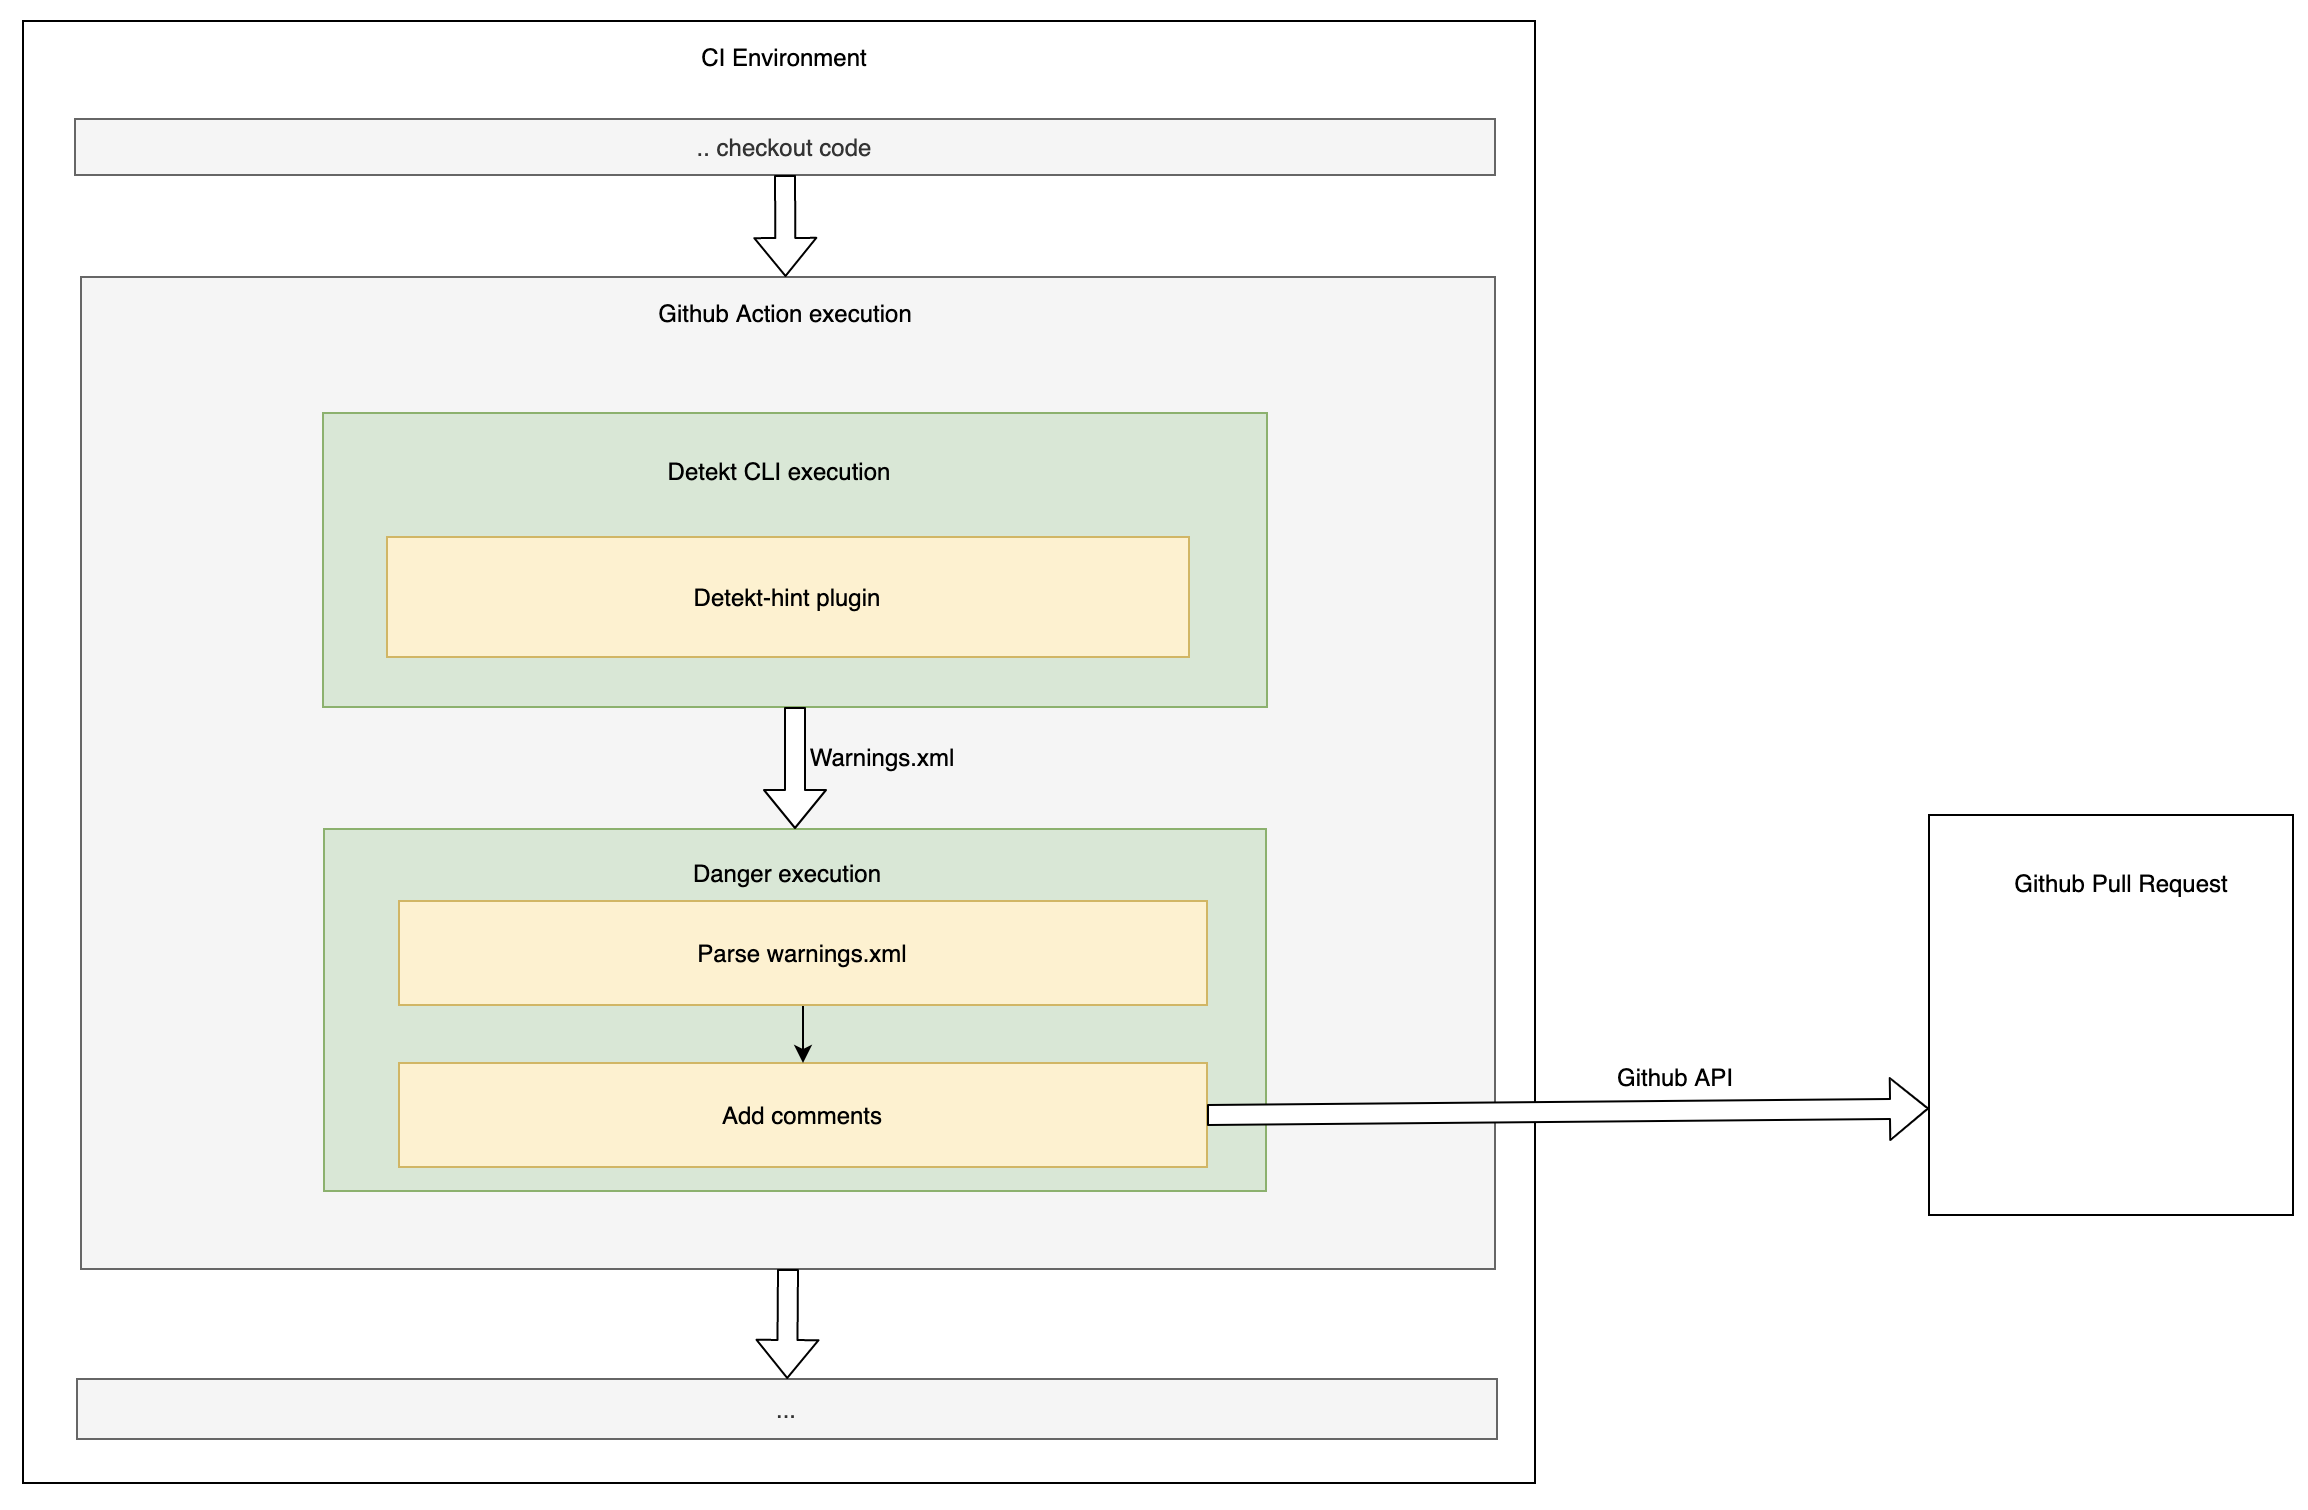
\includegraphics[width=\textwidth]{images/detekt-hint-execution.png}
    \caption{The overall execution flow and the components of the developed solution.}
    \label{fig:integration}
\end{figure}

\cleardoublepage
\chapter{Discussion, further work and conclusion}
\label{discussion}
% Start by rewriting the research questions.
In this chapter we will answer the research questions and give our interpretations, before discussing the impact of our work, its limitations and some recommendations for future research and development. The chapter ends with a conclusion of the study.

\section{Answering the research question}

The research question was as following: \textbf{How to create a tool for \gls{ddpv} that is integrated in the developer workflow without suffering from noise by false-positives?}
The results tell us that by extending a tool for static code analysis, and integrating it with another tool adding comments on \gls{pr} - a tool for \gls{ddpv} can be created. The two identified requirements with utmost importance when developing a tool for \gls{ddpv} is as following. First, it needs to have as accurate rules as possible for \gls{ddpv}. This requires extensive insight into design principles and the architecture and design of software systems. Secondly, for supporting the rules, the integration adding comments to the \gls{pr} needs additional features and mechanisms for reducing the impact and the amount of false-invocations. Depending on the success of implementing the additional features and mechanisms mentioned in section \ref{evaluation-overall}, the implemented rules for \gls{ddpv} may fit or not into the developed solution. The rules with high or medium accuracy, will most probably suit the approach commenting directly on \gls{pr}'s. For the rules where the amount of noise cannot be reduced to an acceptable amount, another less obtrusive approach is suggested in section \ref{futurework}.

Most developed rules were created to support the detection of \textit{indications} that a design principle was violated. One may therefore question if \gls{ddpv} was actually achieved. The rules did not target the design principles directly due to lack of accurate heuristics. Even when targeting indications of design principle violations, the rate of false-positives was high. This brings up the question if creating a successful tool for directly targeting violations of design principles is feasible. It is unsure if we ever will be able to develop accurate heuristics for directly detecting violations of design principles. That however, does not mean that tools should not support indirect detection of design principles violations. With the developed tool we show that indirect detection of design principle violations is possible, and could be useful. 

%Generally, machines need to be considerably better than humans, for humans to trust and use them. 

%This is one important premise that need to be true for this tool to succeed. It seems logical as reducing the amount of design issues in software will increase its internal quality, thus reducing the total development time. By following this reasoning, as long as the positive impact of the true-positives are greater than the negative impact from the false-positives, the tool will contribute to reduced development time. From the evaluation of the tool, it seems like this assumption was false, at least to a certain degree. Inspection of the rule invocations found true-positives, and based on what we know about internal quality and its importance for reducing the total development time it is unlikely that the false-positives would take more time to sort out than the positive impact of fixing the detected design issues. Still, feedback mainly focused on the tool having too many false positives, and that the amount needs to be lowered for the tool to be considered adopted. The reason is probably that most developers dislikes manual tasks, and that sorting out false-positives is a highly manual task, that will get ignored quite fast. Even if the rule is of high importance and would in total impact (considering all the true-positives and the false-positives) improve the internal quality, it will get ignored and dismissed.


\section{Impact}

At current state, the direct impact of the tool are minor. It serves as a proof of concept of a tool that is able to detect some indications of violation of design principles, and that handles the reporting of false-positives in a new way. However, the development of the tool lead to the identification of two central requirements for creating a tool for \gls{ddpv}. The identification of these requirements would be useful for further development. By solving the most major limitations, the tool can be especially useful in teams consisting of developers not familiar with the design principles. As seen in the evaluation, it may contribute to design discussions and learning within the team.

With continued development, adding more rules, improving the accuracy of the rules and implementing more mechanisms for reduction of noise, the tool could potentially have a big impact on the development of maintainable software. It could contribute to an increase in internal quality of developed software, reducing time and development cost. This new approach automatically adding comments to the \gls{pr}, could enable the development of rules for code-analysis with lower accuracy than what is traditionally accepted. This is not limited to design principles, but may also include the development of rules in other domains. For example for the detection of architectural and design-anti patterns.

\section{Limitations}
%Limitations: what can’t the results tell us?
At current state the tool have its limitations. A description of what the results cannot tell us is, and what have limited the results is important to include. By knowing the limitations of the project, one can more accurately decide whether the results are satisfying given the prerequisites, and whether the results could have been better with other prerequisites. 

% Functional limitations
\subsection*{Functional limitations}
First, a solution to the limitation related to GitHub permissions needs to be resolved. This is a purely functional requirement that needs to be resolved for the tool to be fully integrated into open-source workflows. This limitation severely impacted the evaluation-phase and made the integration of the final prototype (which is the key innovative product) untestable by contributors forking the repositories. This limitation were discovered too late, and multiple attempts at possible solutions did not lead to any solutions. Ideally, the integration problems should have been discovered in the process of creating the vertical prototype. Because of this limitation, the tool was mostly evaluated by inspection of generated reports analyzing the code-base, giving the impression that the false-positive rate was much higher than would have been reflected in actual \gls{pr}'s. The results from this evaluation are therefore not as convincing and conclusive as they should have been.

Secondly as previously mentioned, feedback from experienced developers in the open-source community indicated problems related to the tool generating too much noise. The internal evaluation, looking at the number of invocations and analysis of the individual rules supports this finding. Because of this focus on false-positives, the positive impact of the true-positives has received little focus in the evaluation.  

\subsection*{Limitations of the evaluation}
During all the phases of development, many attempts at gathering informants have been done. It has been hard to find experienced developers in Kotlin, that have both the time and will to assist, without getting any benefits. Attempts include advertisements on social media, creating back-links to the GitHub project in multiple GitHub repositories, presenting prototypes at developer meetings, speaking with different companies doing Kotlin development and circulating requests to colleagues in various channels and in open-source communities. The lack of informants have impacted the evaluation and the development of the tool. Given the high requirements for insights into design principles, and the development of heuristics for detecting the violation of them, the lack of informants have affected the quality of developed rules and the evaluation of them. Also, evaluation activities that were initially planned (workshop) could not be completed. The evaluation of the prototypes were therefore mainly based on a few peoples input and perspective, and is therefore a big limitation. The evaluations were mostly informal, and spawned good discussions about \gls{ddpv}. However, more formal and structured evaluations would have been a good addition to get more quantitative results which could complement the informal evaluation.


\subsection*{Limitation of author and methodical choices}
There were some limitations related to the knowledge of the author, and the methodical choices that were taken during development. As the author only have limited experience on design principles and had limited amount of resources to get insights into heuristics for \gls{ddpv} from informants, the results may be showing a rule set with a lower accuracy than what would have been possible. Also, the development phase included a trade-off between focusing on creating enough rules for the tool to provide any value and the accuracy and features for reducing noise. Creating a set of rules became more important, due to a belief that it would be hard to evaluate the tool having only a single rule. In retrospect, spending more effort on experimenting with features reducing generated noise, instead of implementing multiple rules, would have been beneficial for reaching the aims of the research. Also, in hindsight it appeared that the author had an assumption that the more important the rule or design principle is, a higher rate of noise could be tolerated. The results from the evaluation show that this rate of accepted noise was lower than what was initially expected by the author. This may also have contributed to a focus on implementing rules instead of focusing on experimenting on new features for reducing the noise. 

Another limitation was that the early prototypes was focused around the idea of automatically adding comments to pull-requests. The challenge regarding false-positives were presented, but any numbers on its accuracy were not available at that point and may have given the impression that the tool would be more accurate than it actually was. This may have given false-expectations, making many people overly positive to such a tool. Especially targeting the horizontal prototype, more of its width and content dimensions should have been prototyped to better demonstrate the impact of false-positives. It should have included samples that demonstrates the false-positives as well as true-positives. Then, a more realistic view of the tool would have been presented.



\section{Future work}
 As presented above, for the tool to provide any value there are some further research and development that is needed. We will present a list of possible research, features and enhancements that we consider the most important for the success of this tool. 

\begin{itemize}
    \item False-positives and false-negatives are the two biggest opponents of creating a successful tool. Therefore more research on accurate heuristics for \gls{ddpv} is suggested. An approach looking into combining data-sources e.g git history and/or dynamic-software metrics in addition to static analysis of source code, could give more accurate results. 
    
    \item Case study testing the tool, looking for patterns in use over time and receiving structured and rule-specific feedback. Possible effects on team design decisions and discussions.   
\end{itemize}


\subsection*{Development possibilities}
There are mainly two ways of continuing the work on the tool, either by improving the current functionality or by extending it with new functionality. First, some possible solutions to the GitHub Actions limitation is presented. Then, some enhancements and possible new features are presented.


\subsubsection{Possible solutions to GitHub Actions limitations}

\label{possible-solutions}
To understand the limitation that was found one needs to understand how \gls{pr}'s works across forks on GitHub. When a user have their own fork of another repository, build pipelines caused by pull requests to the destination repository runs on the forked repository. Because secrets/tokens private to a repository are not available to forks, one needs to use the \textit{GITHUB\_TOKEN} provided by GitHub for authentication against the GitHub API. Unfortunately this token does not have write access to pull requests against the destination repository when running on a forked repository. Pull requests against the destination repository running on the forked repository will therefore not be able to write comments on the \gls{pr}. Possible solutions to this limitation are: 
\begin{itemize}
    \item A work around using a cron job that runs on the \gls{pr} destination repository. A demo is provided by Yuri Astrakhan \cite{workaround-demo}. 
    
    \item Create an integration working with another \gls{ci} provider like Travis or CircleCI. 
    
    \item A GitHub app that could be installed on the repository. This would require a backend service and could be a good solution going forward and extending the tool with the more involved features presented below.
\end{itemize}

\label{futurework}


\subsection*{Enhancement \& new features}

The usefulness of the tool has mainly been evaluated on the basis of its accuracy. In addition to accuracy, there are other properties that also might be important for a tool to succeed, and that could be improved and enhanced. 

\begin{itemize}
    \item The transparency of the tool. If we know how the tool works, we may tolerate its faults. By opening up the internals of the tool, not treating the tool as a "magic black box", more noise or faults could be accepted.
    
    \item The obtrusiveness of the tool. For the inaccurate rules or design principles that is hard to detect a new approach that makes the developer in control is suggested. For example for the \gls{coi} rule, which is considered the most inaccurate, the \gls{ide} could show the hints when hovering over class-names. This is sketched in figure \ref{fig:a-new-beginning}. This way, the user can get hints on possible design principle violations when the user wants it, making the user in control of when the comments should appear. Such a tool will be less obtrusive. 

\end{itemize}


\begin{figure}[h!]
    \centering
    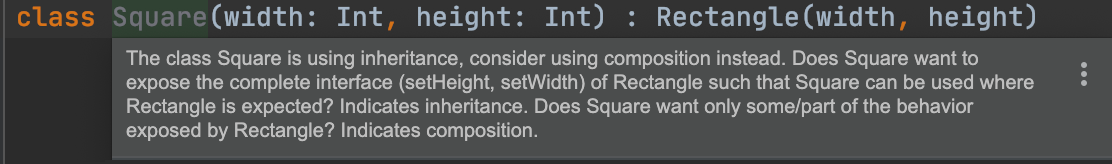
\includegraphics[width=\linewidth]{report/a-new-beginning (2).png}
    \caption{Hovering over the class will present hints on inaccurate rules in an unobtrusive way, directly in the \gls{ide}. Shifts the focus from bot-invocation to user invocation.}
    \label{fig:a-new-beginning}
\end{figure}


One obvious entry point of enhancing the current tool is to enhance the existing rule set, either by enhancing existing rules, or implementing new rules. Some enhancements to the existing rules have been presented in the evaluation of the rules in section \ref{rule-evaluation}. Following are some new rules and enhancements that were considered during development. It was a focus on finding rules that were not targeted in other tools. To the best of the authors knowledge, the below rules is not found in other tools. 

\begin{itemize}
    \item Improving the comments that is posted on the \gls{pr}, giving more in depth suggestions or alternative code changes. Refactoring suggestions and reasoning for required changes.  
    
    \item Command/Query separation principle applied to methods. To promote using methods that either has side effects, or that returns values - not both. 
    
    \item Notify whenever a new enum is created. Misuse of enums is a common design smell.
\end{itemize}


Another entry point for enhancing the tool, which is considered more important is introducing new mechanisms for reducing the amount of noise. A list of enhancements that is considered the most important was presented in section \ref{evaluation-overall}. 

As new enhancements and mechanisms for reducing the noise is introduced the existing rules needs to be reconsidered. For many of the rules a trade-off between rate of false-positives and the rate of false-negatives have been done in favor of the false-positives. This trade-off must be considered together with the mechanisms for reduction of noise. For example for the \gls{isp} rule, the rate of false-positives have been limited by only invoking the rule when empty or methods that only throws exceptions is found. However, this principle can also be broken by adding a method to an interface (interface pollution), without creating any empty implementations. To reduce the rate of false-negatives to zero, one could have invoked the rule every time a new method was added to any interface. This however, would drastically increase the number of false-positives. A decision on reducing the rate of false-positives was therefore made. However, with new mechanisms for reducing the rate of false-positives, such trade-offs should be reconsidered. 

The tool is not limited to just targeting design principles. Rules can be created to support the detection of architectural and design-anti patterns, anti-idiomatic code, or violations of best practices. Another direction for the tool could be as a semi-smart "checklist", reminding developers of double checking aspects of source code that is easily forgotten. For example adding \gls{pr} comments whenever a new file is added or a file is moved, ensuring proper file organization. Or adding comments to ensure that the author of the \gls{pr} left the code-base cleaner than the developer found it - following the Boy Scout Rule \cite{boy-scout}.

\section{Conclusion}
\label{conclusion}


This research aimed to answer how one can create a tool for \gls{ddpv} that is integrated in the developer workflow without suffering from the noise by false-positives. By following the design science methodology, multiple iterations of product development was carried out, and resulted in multiple prototypes and a working \gls{mvp}, using comments on \gls{pr}'s to report possible design issues. The \gls{mvp} was evaluated internally and using the open-source community. 


The results show that using automated comments on \gls{pr} to inform the developer about possible design issues will reduce the noise from false-positives significantly. This will enable the development of rules for \gls{ddpv} with lower requirements on accuracy than what is traditionally accepted. However, the difficulty of \gls{ddpv} creates such big amount of false-positives that further development on mechanisms for reducing the noise, and research on accurate heuristics for \gls{ddpv} is needed.

Initially, it was assumed that increasing the importance of the executed analysis would increase the tolerance for noise. This research shows that the importance of executed analysis will not increase the tolerance for noise drastically. Therefore, when developing a tool for \gls{ddpv} the reduction of noise is of greatest importance. 

To better understand the implications of a tool for \gls{ddpv}, continued research on accurate heuristics and development of supporting mechanisms for reducing the amount of noise is suggested. If successful, a new category of tools supporting the development of maintainable code is possible. This new category of tools, will not only be able to target design principles, but also support the development of rules in other domains where 100\% accuracy could not be achieved. Examples include higher level analysis, including architectural and design anti-patterns detection, or lower level analysis supporting best practices.

\section{Acknowledgments}
\label{acknowledgements}
I would firstly like to thank my supervisor, associate professor Hallvard Trætteberg for his expert advice and dedication during the development and the writing of this masters thesis. Especially, his advice and insights on the topics of academical writing and software development has been useful, together with his efforts in helping out with getting in touch with possible informants.

Thanks to JavaBin Trondheim and the participants that were present and gave feedback during the presentation of the prototype. Also, thanks to the participants of the semi-structured interview and the contributors of the open-source projects where Detekt-hint was integrated and tested. Lastly, i would like to thank Eirik Vale Aase for his dedication and for being an active sparring partner during the development of this masters thesis.

\printglossary[type=\acronymtype]
\printbibliography

\appendix
\label{appendix}
\clearpage
\chapter{Appendix}

\section{Horizontal prototype}
\label{horizontal-prototype-images}

\begin{figure}[h!]
    \centering
    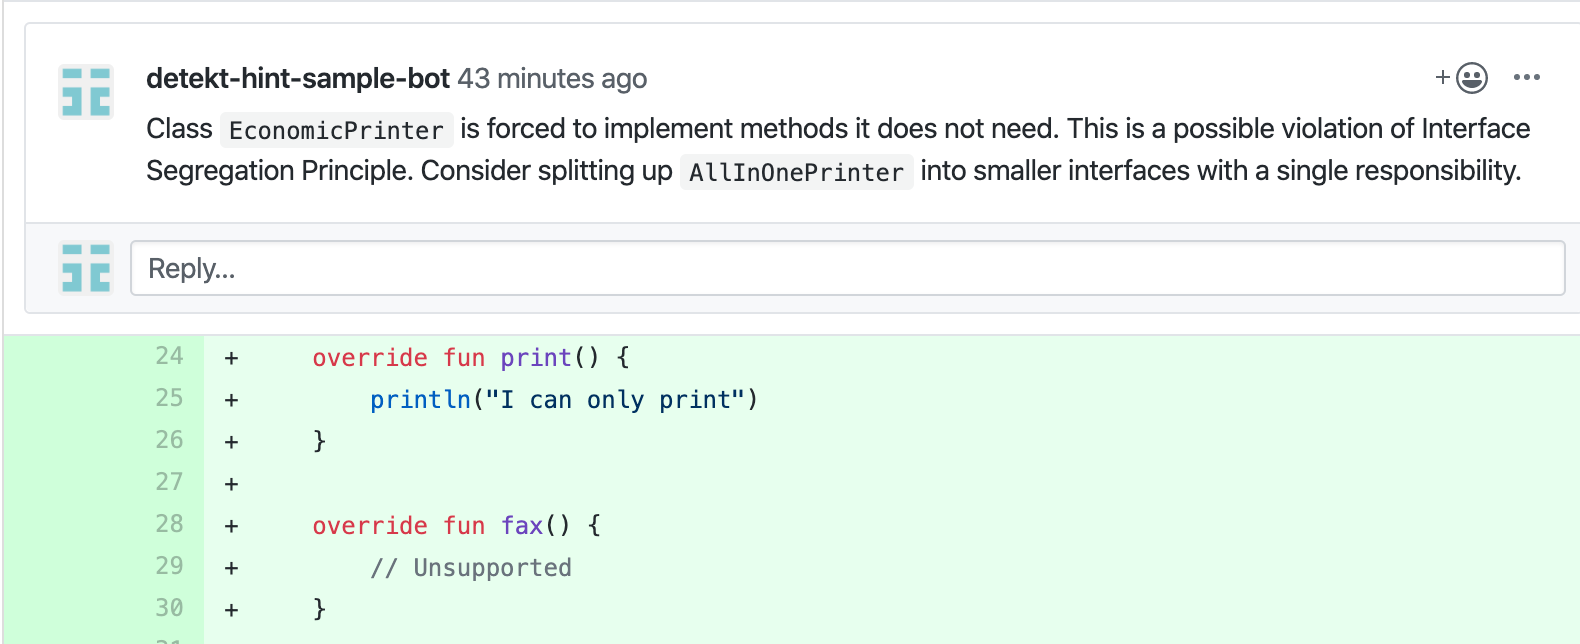
\includegraphics[width=\textwidth]{../images/comment_isp.png}
    \caption{Screenshot of the horizontal prototype showing the \gls{isp} rule. It has detected an empty method, which is a sign of violating the \gls{isp}. In this case the \texttt{EconomicPrinter} implements methods from \texttt{AllInOnePrinter} which it does not need. A solution would be to define separate interfaces for each of the responsibilities (e.g \texttt{Printable, Faxable, Scanable}) and let the concrete implementations of printers implement the interfaces they need.}
    \label{fig:isp}
\end{figure}


\begin{figure}[h!]
    \centering
    \includegraphics[width=\textwidth]{../images/comment_lackOfCohesion.png}
    \caption{Screenshot of the horizontal prototype showing the \gls{lcom} rule, with a visual representation of the lack of cohesion. The figure shows which fields that are referenced from each of the methods in the class. In this case all the methods of the class references their own separate field. This indicates that each of the methods and corresponding fields have separate responsibilities within the class. This would therefore be an indication of violating the \gls{srp}.}
    \label{fig:lcom}
\end{figure}


\begin{figure}[h!]
    \centering
    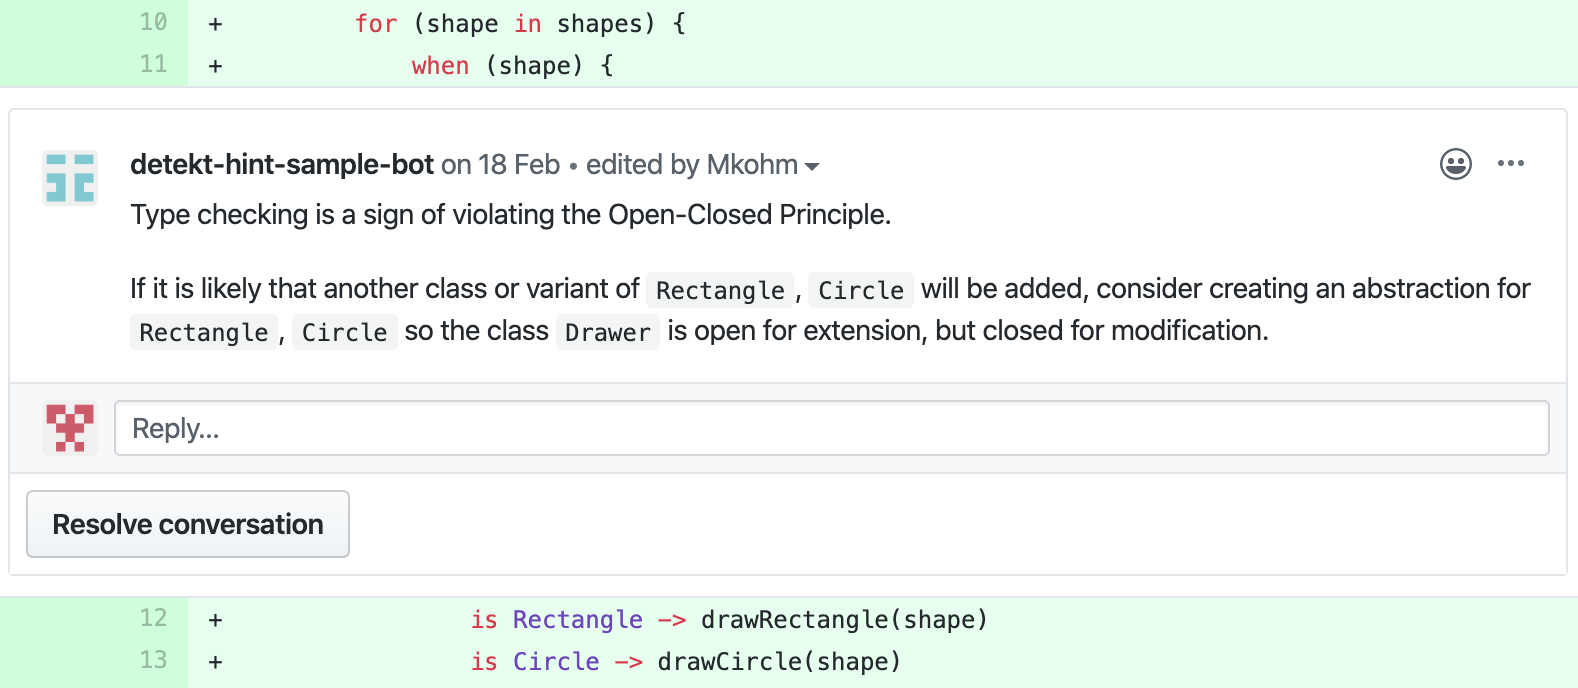
\includegraphics[width=\textwidth]{images/comment_ocp2.png}
    \caption{Screenshot of the horizontal prototype that shows the \gls{ocp} rule, using a simple program for drawing shapes. In this case the rule detected checking of concrete implementations to control flow. The rule suggests creating an abstraction for \texttt{Rectangle}, \texttt{Circle} (e.g an interface \texttt{Shape} with a \texttt{draw} method that all \texttt{Rectangle} and \texttt{Cirle} should implement) such that eventual new shapes added to the program would not need to modify existing code. }
    \label{fig:ocp}
\end{figure}


\begin{figure}[h!]
    \centering
    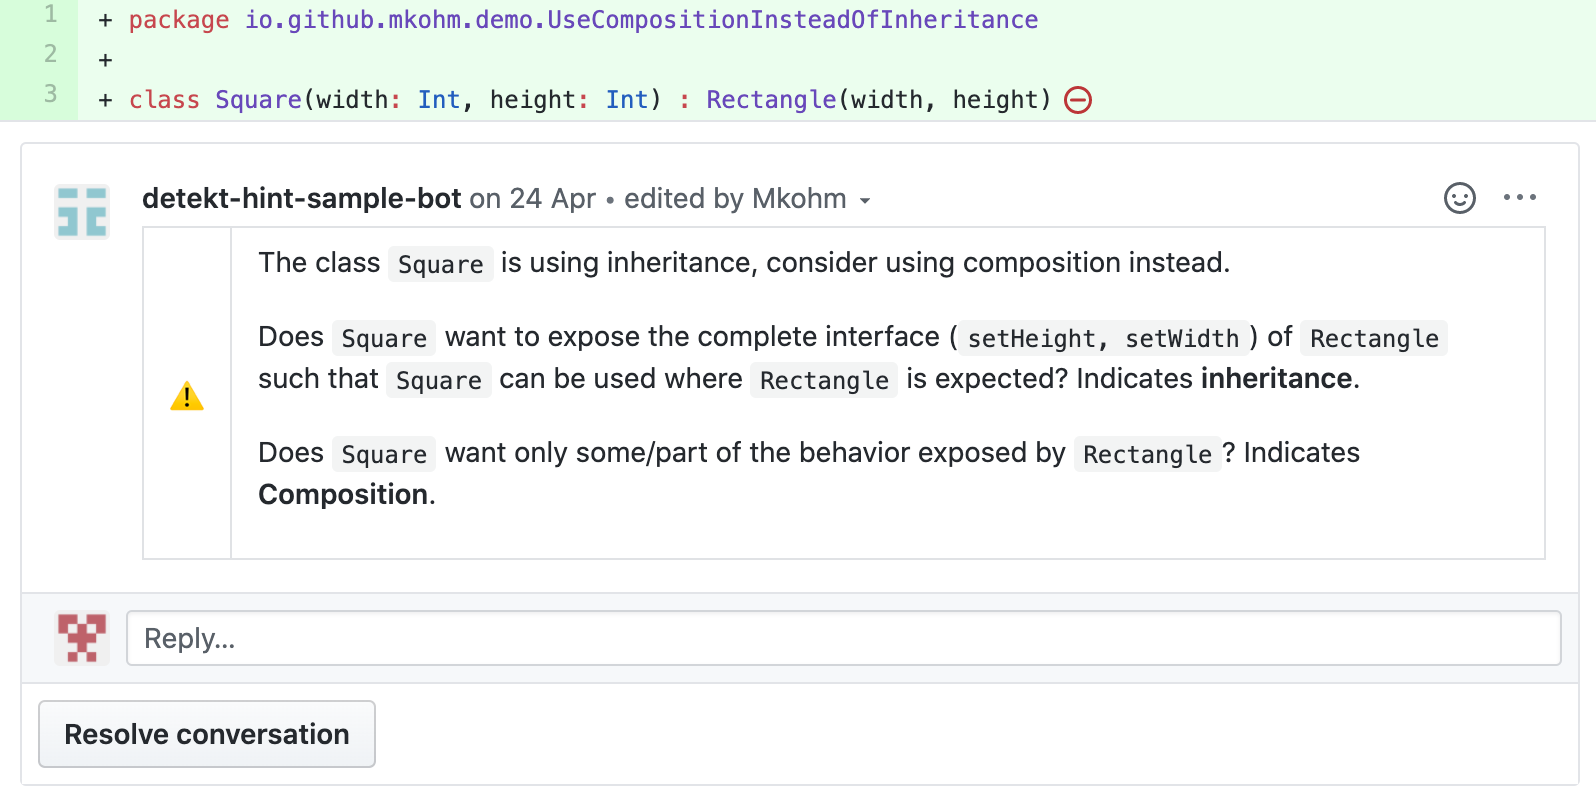
\includegraphics[width=\textwidth]{images/horizontal-prototype-coh.png}
    \caption{Screenshot of the horizontal prototype that shows the \gls{coi} rule. The rule suggests the use of composition instead of inheritance, and helps testing if the classes adheres to the \gls{lsp}. In this case, the classical Square - Rectangle problem is presented. \texttt{Square} should not be derived from \texttt{Rectangle} as it would violate the \gls{lsp}. \texttt{Square} does not functionally behave like \texttt{Rectangle} as squares by definition have the same width and height. \texttt{Rectangle} should have two independent methods for changing its size, but clearly these methods is not appropriate for the \texttt{Square}. }
    \label{fig:liskov}
\end{figure}

\clearpage

\section{Semi-structured interview schema}
\label{semi-structured-interview-schema}
\subsubsection*{Participant number:} What is the number of the participant.
\subsubsection*{Background:} What is the participants background. Experience with software architecture? Knows and uses design principles? Experience with Kotlin?
\subsubsection*{Presentation of rules - For each rule}
\begin{enumerate}
    \item Present the rule. 
    \item Make sure the participant understands the importance of the rule.
    \item When will the rule give a warning?
    \item When will the rule incorrectly give a warning? Will it report false-positives too often? Suggestions on how to reduce the amount?
    \item How much context is needed? Shorter or longer comments? Should include suggestions on possible solutions? Is the comment understandable? Something missing?
\end{enumerate}

\subsubsection*{Other} 
- When reviewing code, what do you think is tedious, and could it be automated?
- Are there any rules/principles missing?

\clearpage
\section{Semi-structured interview results}
\label{horizontal-prototype-interview-results}

\textbf{Participant number:} 1 \newline
\textbf{Background:} Studies computer science at \gls{ntnu} with a specialization in computers and systems software. Has experience with developing apps for iOS and web and back-end development. Interested in Software Architecture and writing software of high quality. \\
\textbf{Experience with design principles:} Some \\\\

\noindent \gls{coi}: Could be useful, but potentially have too many false positives. For testing the participant often creates Mock objects that inherits from the class he wants to Mock, and then overrides methods. The participant think there is too few cases where this rule will be useful. Suggestions: Reduce the amount of positives by disabling checks for classes with names; Mock. User could specify which class names or a pattern to ignore. Should revisit sentence number two about composition, it could be misleading.\\\\

\noindent LCOM1: Very useful because calculating such a value is'nt something you do while coding. Positive that you can change the threshold of the rule. Suggestion: Which fields and methods could i extract? A comment that suggests a solution. \\\\

\noindent LCOM2 (With refactoring visualization): Look more at further analysis to find out what can be extracted. Look into dependencies between function calls as well. Diagram looks cool, but does not give any more value than some plain text explaining what can be extracted. \\\\

\noindent \gls{ocp}: Somewhat useful. Should have a more specific comment saying if you are doing enum switching or instanceOf checking. \\\\

\noindent \gls{isp}: Could be useful. Suggestion to count number of usages of calls in the interface to see which method calls that is not used by any of the classes that implement the interface. \\\\

\noindent Other: Tools for detecting complicated expressions that can be extracted out as a separate method with a descriptive name. Blocks of code should be extracted out as separate methods so that lines of code that belongs together has its own scope. 
\clearpage


% Netlight
\noindent\textbf{Participant number:} 2 \newline
\textbf{Background:} Works as a software developer for Netlight, 2 years of professional developer experience. Experienced with Kotlin development and with architecture and design of software systems.\\
\textbf{Experience with design principles:} Yes \\\\

\noindent \gls{coi}: Positive about the rule, but is concerned about not showing warnings when deriving from third party libraries. This is a case where one also should think about using composition instead of inheritance. Suggests to remove this logic, and instead provide configuration options for packages that should not be reported as violations when derived from.  \\\\

\noindent \gls{lcom}: Nothing special. \\\\

\noindent \gls{ocp}: Useful for both instance of checking and enum switching. Enums in Kotlin are powerful, so switching on them is in many cases not needed and polymorphism is used instead.\\\\

\noindent \gls{isp}: Could be useful. May need to handle TODO's specially. \\\\

\noindent Other: In general positive to the tool, and think it has potential. Good that it is easy to ignore warnings, with just a click. It needs more rules before considering using it. For example including detection of Java anti-patterns and ensuring that Kotlin code is idiomatic. For example static methods and places where data-classes could be used. The tool could be used as "training wheels" in a team, where one gradually could disable more rules to not create unnecessary noise in the development.

\clearpage
\section{Final prototype}
\label{final-artifact}
\begin{figure}[h!]
    \centering
    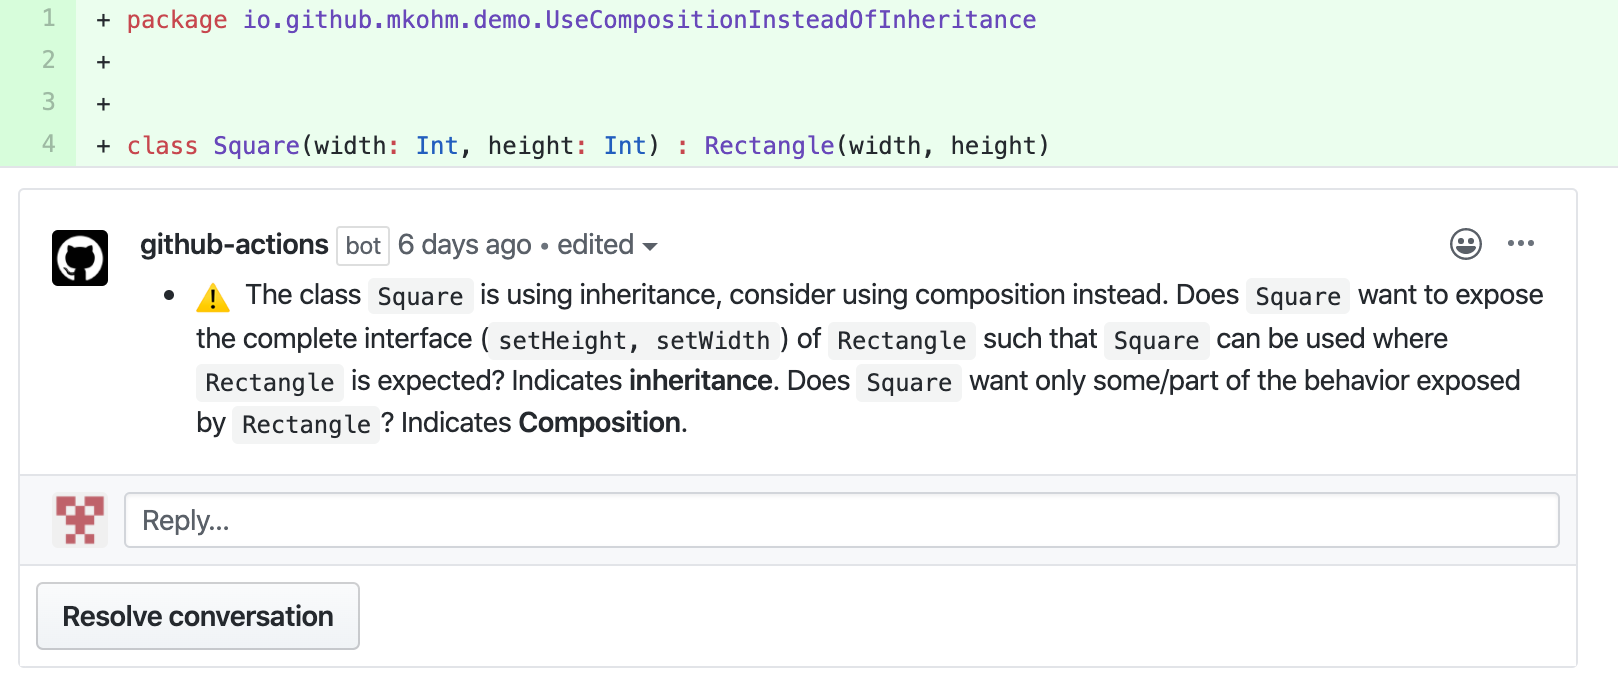
\includegraphics[width=\textwidth]{images/final_coh.png}
    \caption{Screenshot of the final prototype that shows the \gls{coi} rule. The rule suggests the use of composition instead of inheritance, and helps testing if the classes adheres to the \gls{lsp}. In this case, the classical Square - Rectangle problem is presented. \texttt{Square} should not be derived from \texttt{Rectangle} as it would violate the \gls{lsp}. \texttt{Square} does not functionally behave like \texttt{Rectangle} as squares by definition have the same width and height. \texttt{Rectangle} should have two independent methods for changing its size, but clearly these methods is not appropriate for the \texttt{Square}.}
\end{figure}

\begin{figure}[h!]
    \centering
    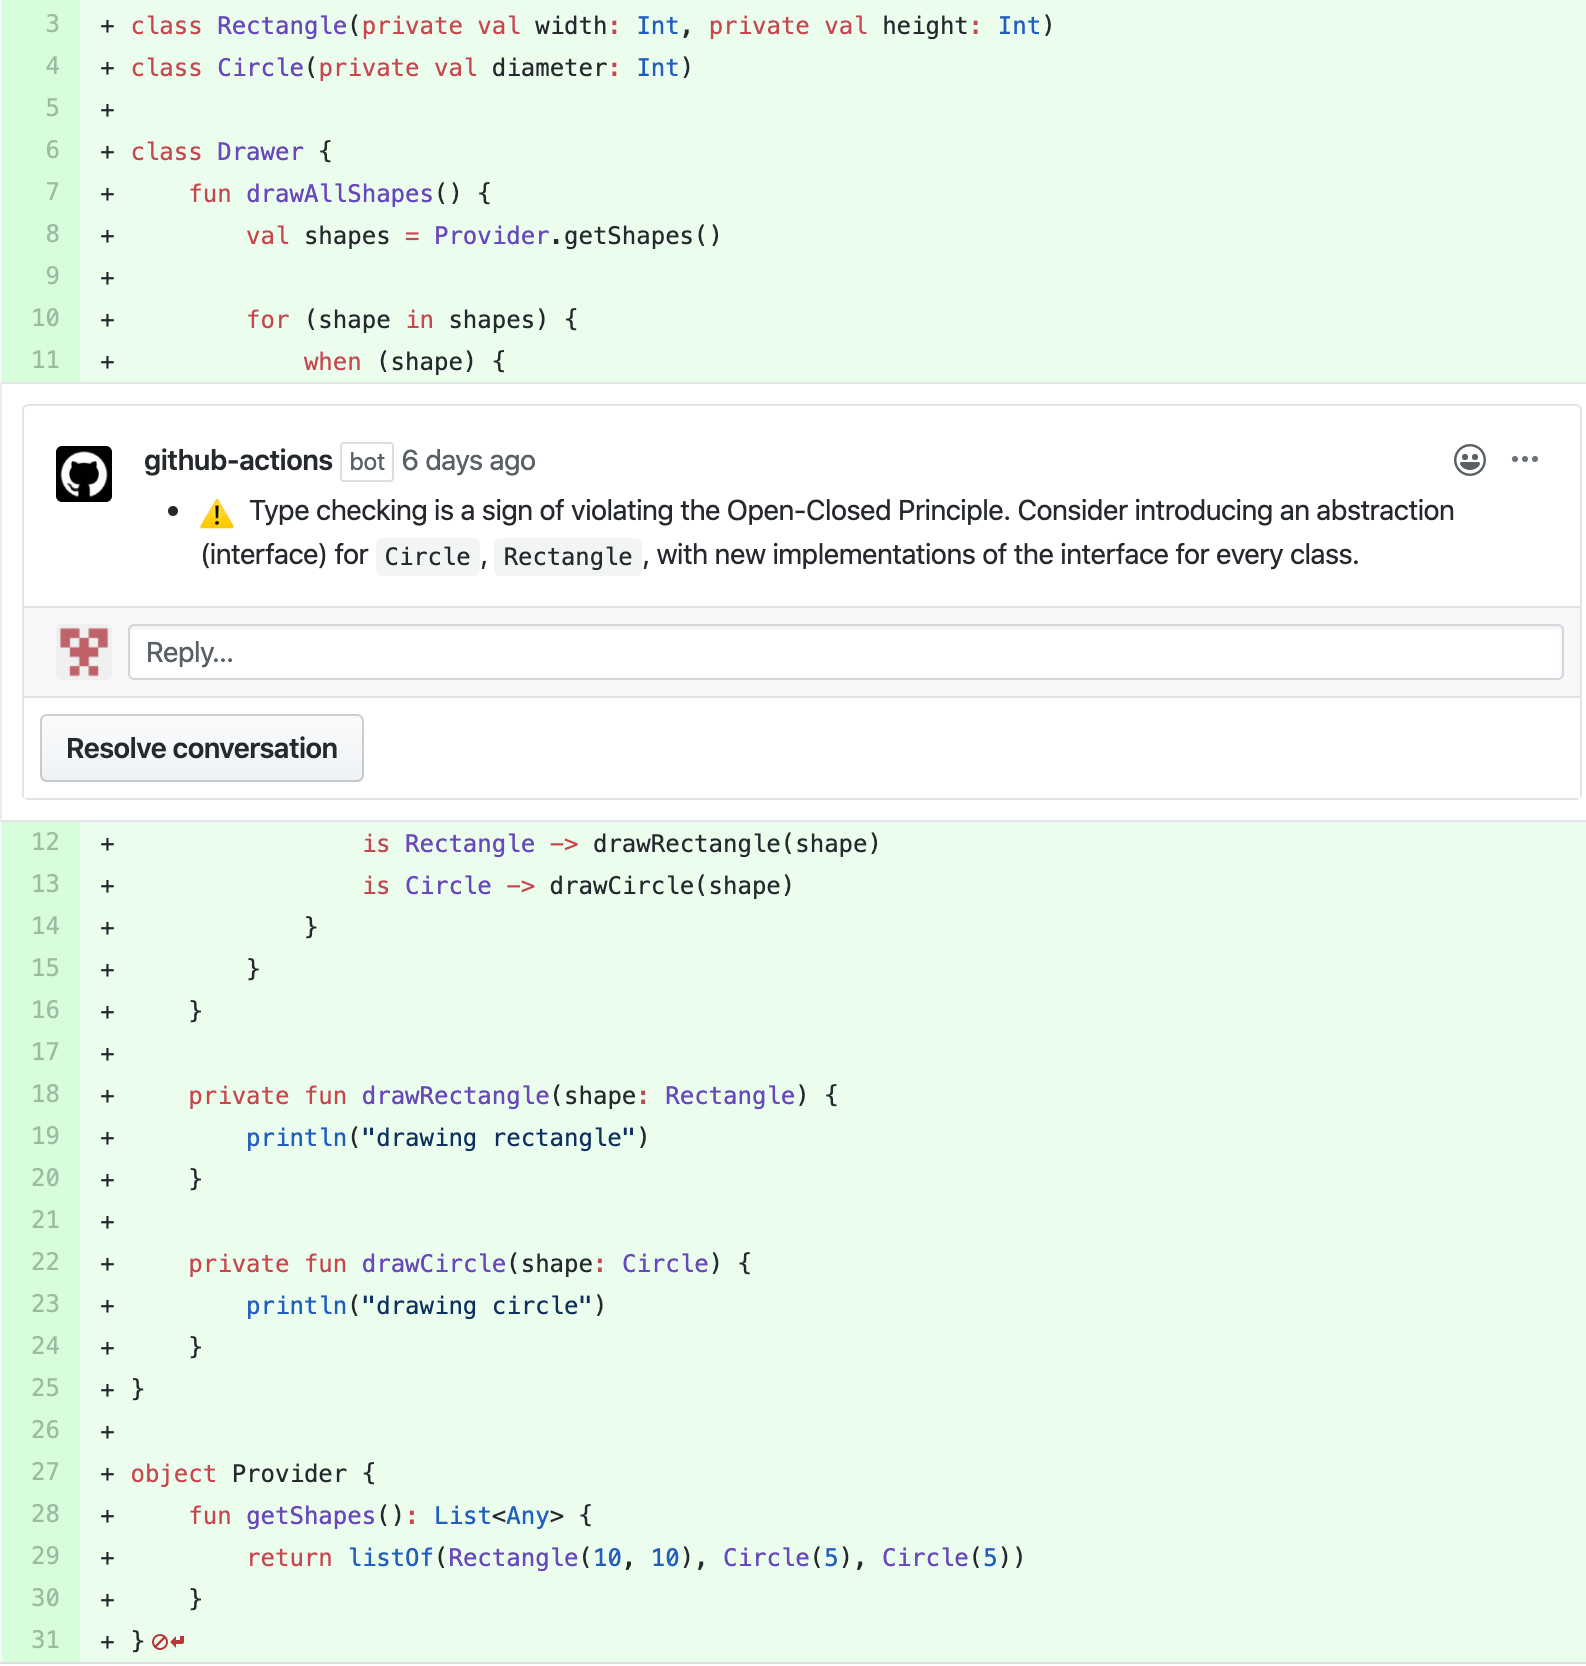
\includegraphics[width=\textwidth]{images/final_ocp.png}
    \caption{Screenshot of the final prototype that shows the \gls{ocp} rule, using a simple program for drawing shapes. In this case the rule detected checking of concrete implementations to control flow. The rule suggests creating an abstraction for \texttt{Rectangle}, \texttt{Circle} (e.g an interface \texttt{Shape} with a \texttt{draw} method that all \texttt{Rectangle} and \texttt{Cirle} should implement) such that eventual new shapes added to the program would not need to modify existing code.}
\end{figure}

\begin{figure}[h!]
    \centering
    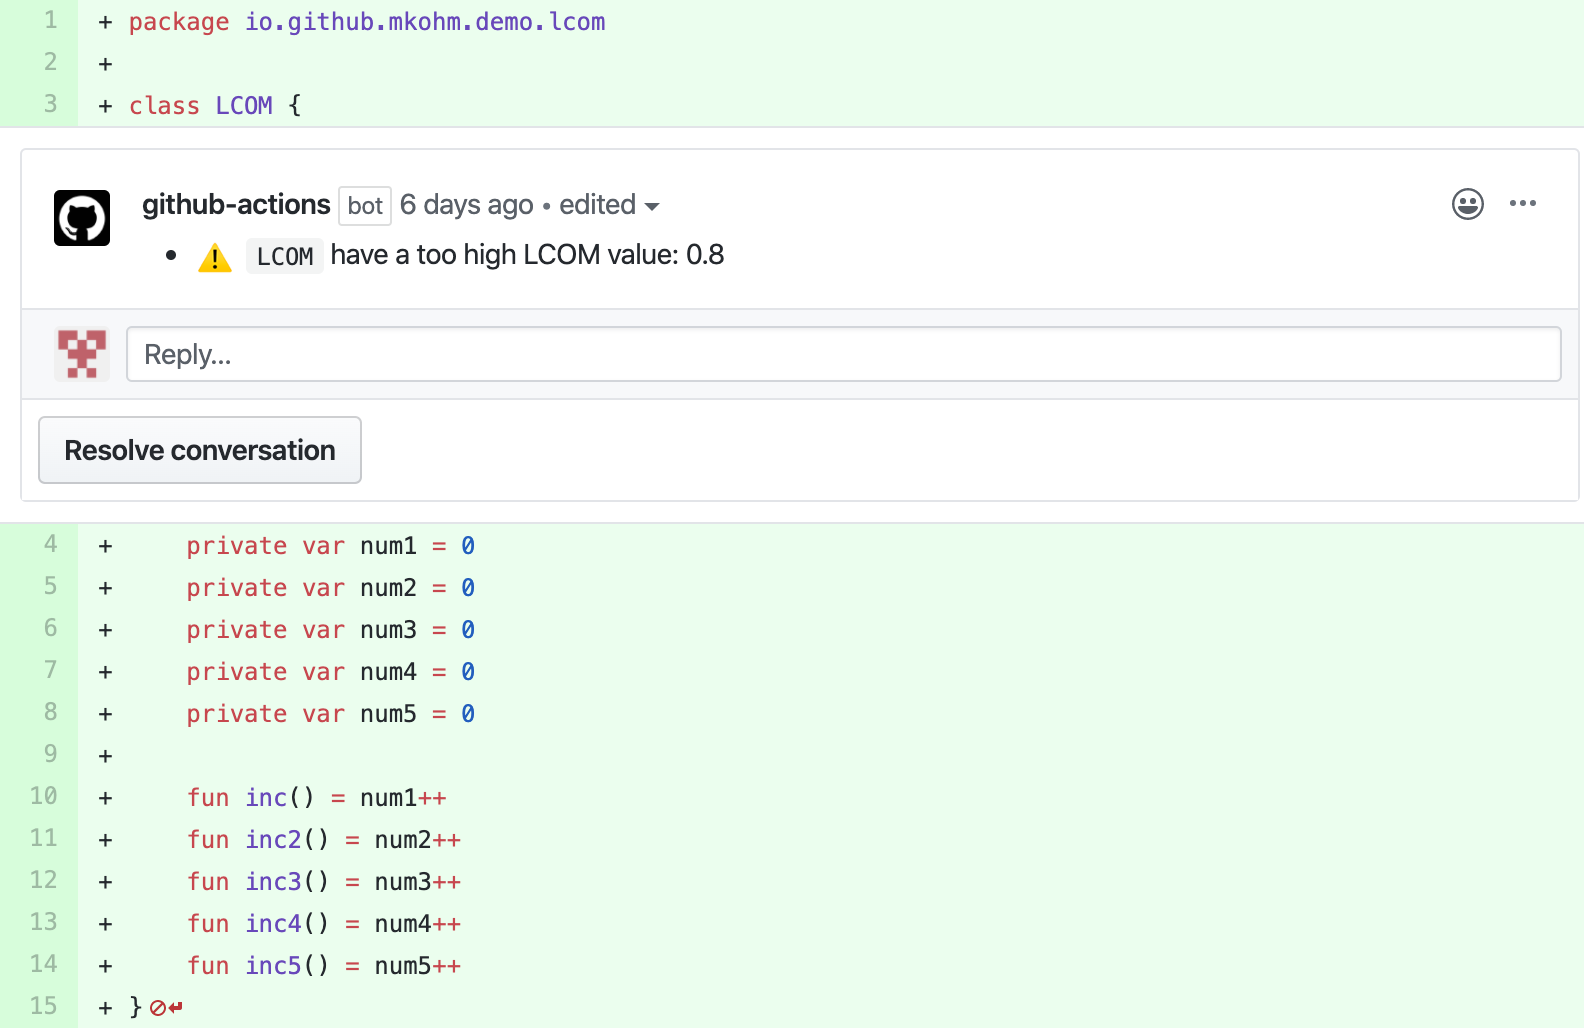
\includegraphics[width=\textwidth]{images/final_lcom.png}
    \caption{Screenshot of the final prototype showing the \gls{lcom} rule. This is an indication of violating the \gls{srp}, due to low cohesion in the class. In this case, each of the methods reference their own field, telling us that there is no relationship between the different methods, and that they don't need to exist in the same class.}
\end{figure}

\begin{figure}[h!]
    \centering
    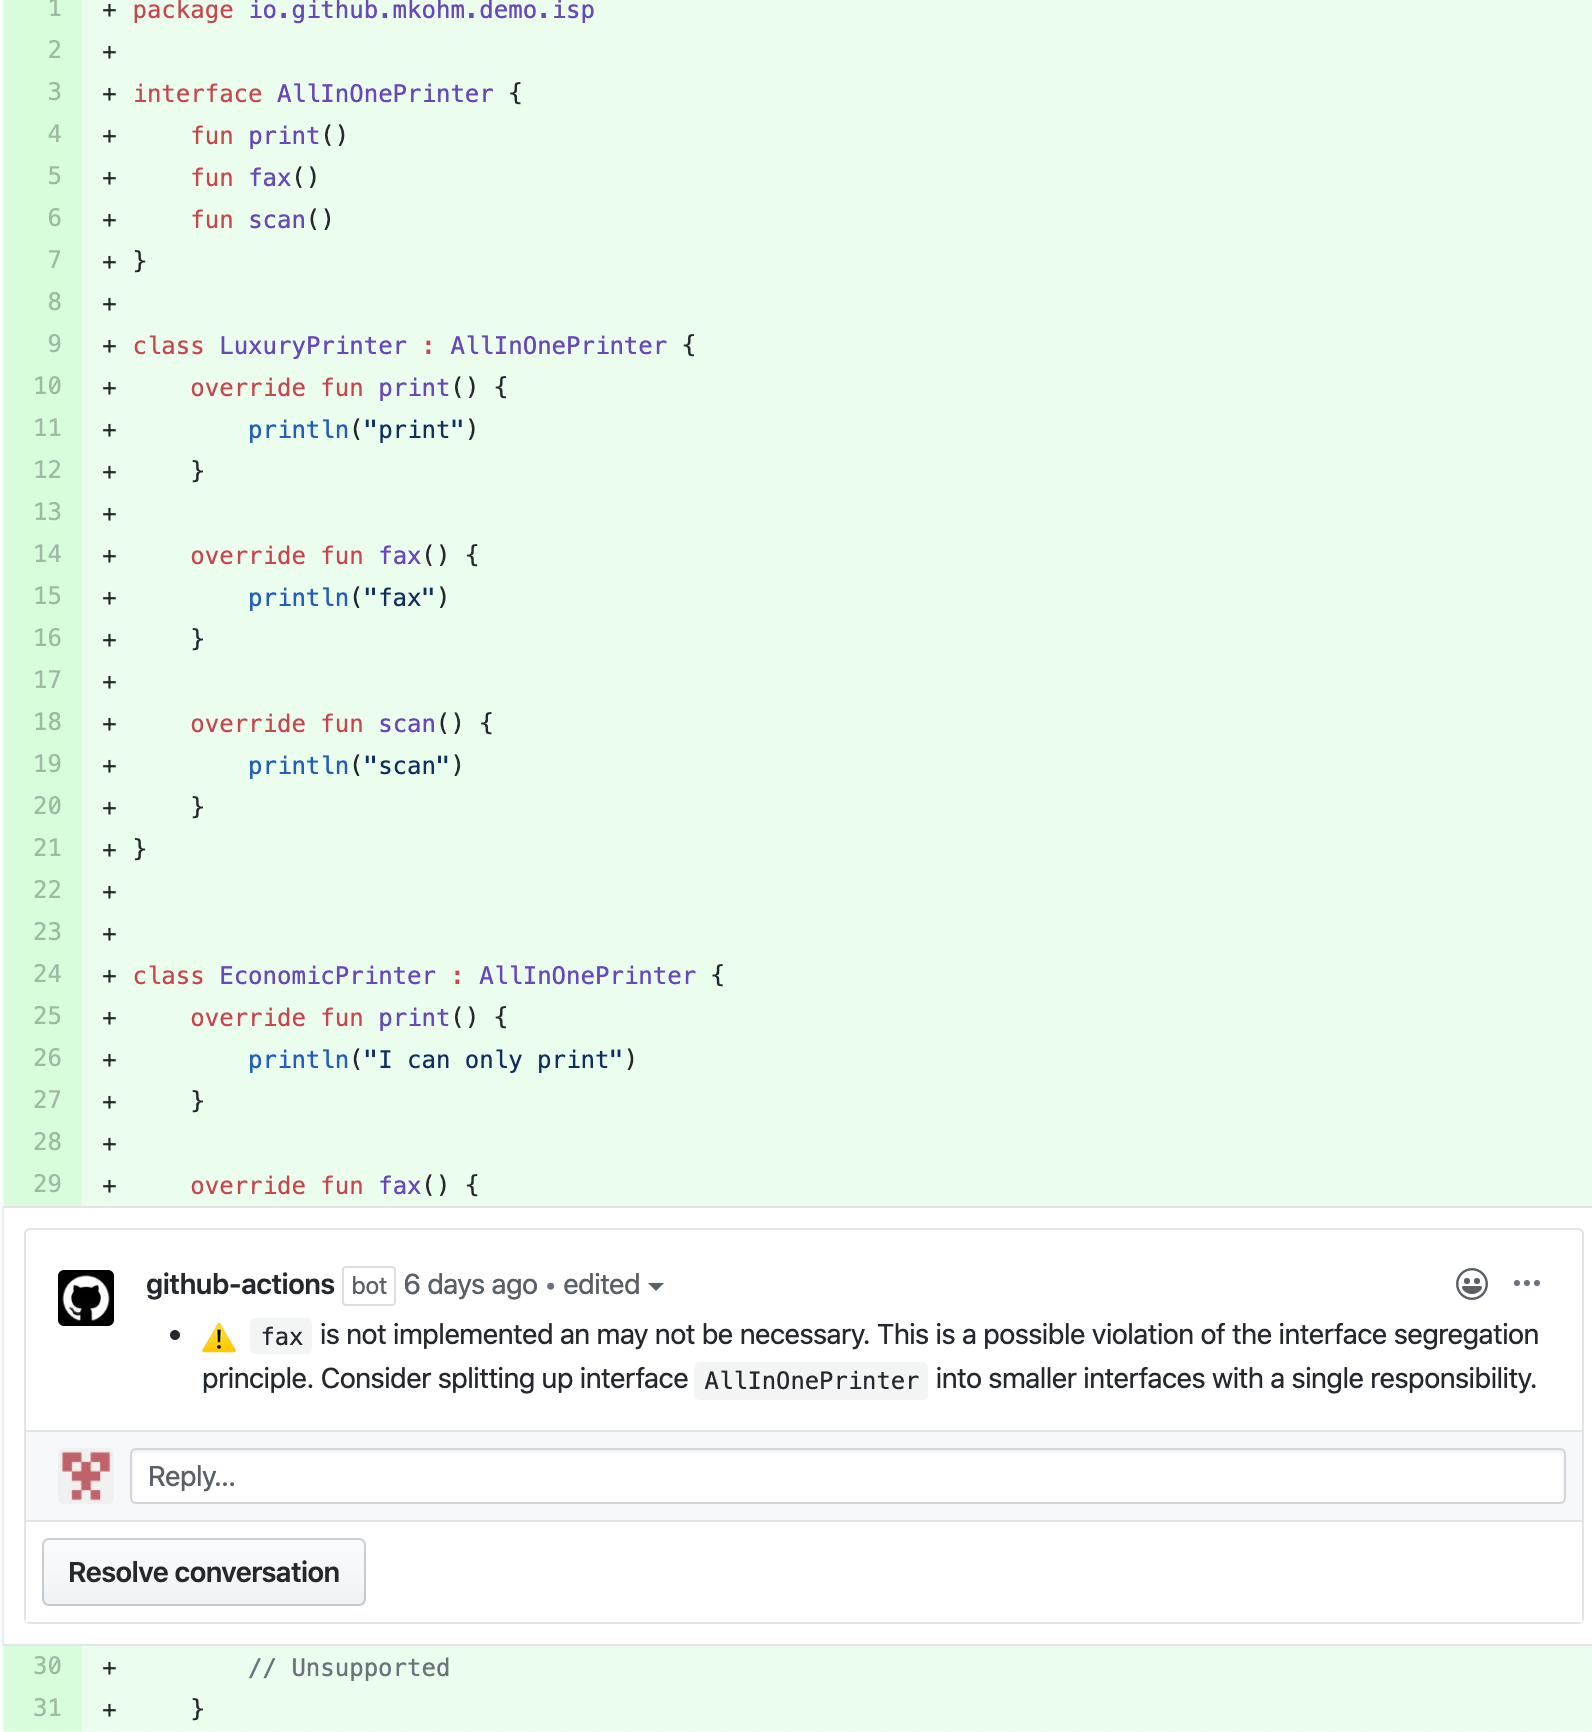
\includegraphics[width=\textwidth]{images/final_isp.png}
    \caption{Screenshot of the final prototype showing the \gls{isp} rule. It has detected an empty method, which is a sign of violating the \gls{isp}. In this case the \texttt{EconomicPrinter} implements methods from \texttt{AllInOnePrinter} which it does not need. A solution would be to define separate interfaces for each of the responsibilities (e.g \texttt{Printable, Faxable, Scanable}) and let the concrete implementations of printers implement the interfaces they need.}
\end{figure}



\end{document}